
\documentclass[10pt,a4paper]{article}

% ============== PACKAGES ==============
\usepackage[utf8]{inputenc}
\usepackage[T1]{fontenc}
\usepackage{geometry}
\usepackage{graphicx}
\usepackage[hyphens]{url}
\usepackage{xurl} % smarter URL breaking
\usepackage[colorlinks=true, breaklinks=true, urlcolor=blue, linkcolor=blue, citecolor=blue]{hyperref}
\usepackage{fancyhdr}
\usepackage{hyperref}
\usepackage{titlesec}
\usepackage{xcolor}
\usepackage{amsmath}
\usepackage{amssymb}
\usepackage{booktabs}
\usepackage{caption}
\usepackage{subcaption}
\usepackage{pgfplots}
\pgfplotsset{compat=1.18}
\usepackage{tikz}
\usetikzlibrary{positioning, arrows.meta, shapes.geometric}
\usepackage{enumitem}
\usepackage{times} % Similar to Google's font

% ============== PAGE SETUP ==============
\geometry{
    a4paper,
    left=2.5cm,
    right=2.5cm,
    top=3cm,
    bottom=2.5cm,
    footskip=1cm,
    headheight=1.5cm,
    headsep=0.5cm
}

% ============== HYPERLINK COLORS ==============
\hypersetup{
    colorlinks=true,
    linkcolor=blue,
    citecolor=blue,
    urlcolor=blue,
    pdftitle={The Open Intelligence Paradigm},
    pdfauthor={Your Name}
}

% ============== HEADER/FOOTER SETUP ==============
\pagestyle{fancy}
\fancyhf{} % Clear all headers and footers

% First page header (will be overridden)
\fancypagestyle{firstpage}{
    \fancyhf{}
    \fancyhead[L]{\raisebox{-0.6cm}{
\includegraphics[height=1.2cm]{logo.png}}} % Bigger logo, lowered
    \fancyhead[R]{\raisebox{-0.1cm}{2025-10-5}} % Slightly lowered date
    \fancyfoot[C]{\rule{0.9\textwidth}{0.4pt}}
    \fancyfoot[R]{\thepage}
    \renewcommand{\headrulewidth}{0pt}
    \renewcommand{\footrulewidth}{0pt}
}

% Subsequent pages header
\fancyhead[L]{}
\fancyhead[C]{\small\textit{The Open Intelligence Paradigm: A Quantitative Analysis}}
\fancyhead[R]{}
\fancyfoot[C]{\rule{0.9\textwidth}{0.4pt}}
\fancyfoot[R]{\thepage}
\renewcommand{\headrulewidth}{0.4pt}
\renewcommand{\footrulewidth}{0pt}

% ============== SECTION FORMATTING ==============
\titleformat{\section}
  {\normalfont\Large\bfseries}{\thesection.}{0.5em}{}
\titleformat{\subsection}
  {\normalfont\large\bfseries}{\thesubsection}{0.5em}{}
\titleformat{\subsubsection}
  {\normalfont\normalsize\bfseries}{\thesubsubsection}{0.5em}{}

\titlespacing*{\section}{0pt}{12pt}{6pt}
\titlespacing*{\subsection}{0pt}{10pt}{5pt}
\titlespacing*{\subsubsection}{0pt}{8pt}{4pt}

% ============== CUSTOM COMMANDS ==============
\newcommand{\papertitle}[1]{%
    {\LARGE\bfseries #1}%
}

\newcommand{\papersubtitle}[1]{%
    {\large\textit{#1}}%
}

\newcommand{\authorlist}[1]{%
    {\normalsize #1}%
}

% ============== DOCUMENT START ==============
\begin{document}

\thispagestyle{firstpage}

% Top line under logo/date
\noindent\rule{\textwidth}{0.4pt}

\vspace{1em}

% ============== TITLE ==============
\begin{center}
\papertitle{The Open Intelligence Paradigm: A Quantitative Analysis of Architectural Openness and Computational Utility in Contemporary AI Systems}

\vspace{0.5em}

\papersubtitle{Why Decentralized AI Infrastructure Will Dominate the Next Decade}

\vspace{1.5em}

% ============== AUTHORS ==============
\authorlist{Shiro Oni \\ }


\vspace{0.5em}



\end{center}

\vspace{1em}

% Bottom line before content
\noindent\rule{\textwidth}{0.4pt}

\vspace{1em}

% ============== ABSTRACT ==============
\begin{abstract}
\noindent
This technical report presents a quantitative framework for evaluating the relationship between architectural openness and computational performance in contemporary artificial intelligence systems. The central question examined is whether decentralized, open-source AI architectures can achieve competitive utility compared to proprietary closed-source systems. We introduce the Openness-Utility Index, a multidimensional scoring methodology that systematically assesses AI systems across ten distinct criteria spanning model transparency, infrastructure decentralization, governance structures, factual retrieval accuracy, reasoning capability, and multi-agent orchestration performance. 

Through systematic analysis of publicly available benchmark results from FRAMES (factual retrieval and multi-hop reasoning), SimpleQA (short-form factuality), and SEAL-0 (search-augmented reasoning under adversarial conditions), we evaluate six major AI systems: Sentient's Open Deep Search and ROMA frameworks, OpenAI's GPT-4o, Anthropic's Claude 3.5 Sonnet, Perplexity's answer engine, and DeepSeek V3. Our analysis reveals that Sentient represents the first documented case of an AI system achieving both maximum architectural openness (10/10 on our scoring framework) and competitive computational utility (8.0/10), with published benchmark results showing 75.3 percent accuracy on FRAMES and 45.6 percent on SEAL-0, compared to estimated performance ranges of 60-65 percent and 17-36 percent respectively for competing systems.

To contextualize these findings, we examine historical adoption patterns in open-source infrastructure technologies, documenting Linux's trajectory to 96.3 percent server market dominance over 17 years, Android's capture of 73.9 percent mobile market share within 5 years, and Kubernetes' achievement of 96 percent enterprise adoption in 5 years. This historical analysis establishes an empirical basis for projecting that modern open-source projects in rapidly evolving technical domains achieve market dominance within 5 to 7 years. We discuss the architectural innovations enabling Sentient's performance, including cryptographic model fingerprinting for provenance tracking, distributed compute orchestration, and community-governed alignment mechanisms. The report concludes by examining implications for AI development practices, enterprise adoption strategies, and governance frameworks in an evolving landscape where the traditional trade-off between openness and performance may no longer hold.
\end{abstract}

\vspace{1em}

\noindent\textbf{Keywords:} Open-source AI, Decentralized Intelligence, AGI Infrastructure, Sentient Protocol, Benchmark Analysis, AI Governance

\vspace{1em}

\noindent\rule{\textwidth}{0.4pt}

% ============== IMPORT SECTIONS ==============

% ============== SECTION 1: INTRODUCTION ==============

\section{Introduction}

The artificial intelligence industry has entered a period of unprecedented market concentration. As of October 2025, OpenAI commands a valuation of 500 billion dollars following its latest secondary share sale, establishing itself as the world's most valuable private company \cite{openai2025}. Anthropic reached a post-money valuation of 183 billion dollars through its Series F funding round in September 2025, with annual recurring revenue exceeding 5 billion dollars \cite{anthropic2025}. These valuations reflect extraordinary investor confidence in proprietary AI systems, yet they simultaneously raise fundamental questions about the sustainability and desirability of increasingly centralized control over intelligence infrastructure.

This concentration of AI capabilities within a small number of closed-source organizations creates several interconnected challenges. First, compute resource requirements have created effective barriers to entry, with training costs for frontier models reaching hundreds of millions of dollars and requiring access to tens of thousands of specialized processors. Second, the opacity of proprietary systems makes independent verification of safety claims, alignment methodologies, and performance characteristics functionally impossible for external researchers. Third, regulatory frameworks such as the European Union AI Act and various national executive orders are being designed in an environment where regulators must rely primarily on self-reported information from the organizations they seek to regulate.

\subsection{The Centralization Crisis in Modern AI}

The current AI landscape exhibits market dynamics that differ substantially from other technology sectors. OpenAI's 500 billion dollar valuation represents a 67 percent increase over its 300 billion dollar Series F valuation from March 2025, achieved in merely seven months \cite{openai2025}. Anthropic's trajectory shows similar acceleration, growing from a 61.5 billion dollar post-money valuation to 183 billion dollars \cite{anthropic2025}. Additional major players include xAI with valuations ranging between 177 and 200 billion dollars depending on reporting sources, and Perplexity AI reaching 20 billion dollars in September 2025 despite having launched its core product only two years prior \cite{perplexity2025}.

These valuations aggregate to a total closed-source AI market value exceeding 880 billion dollars among just four major organizations. The capital intensity of this industry segment creates natural monopolistic tendencies. Training frontier models requires not only substantial financial resources but also access to compute infrastructure that remains concentrated among a small number of cloud providers and chip manufacturers. This concentration raises concerns about equitable access to AI capabilities, particularly for academic researchers, smaller organizations, and developers in regions with limited access to compute resources.

The architectural opacity of closed systems compounds these access concerns. Contemporary leading AI systems operate as black boxes, with their training data, model architectures, fine-tuning processes, and alignment techniques remaining proprietary. While organizations like OpenAI and Anthropic publish selected benchmarks and system cards, independent researchers cannot verify these claims or conduct their own evaluations using identical methodologies. This opacity creates fundamental challenges for AI safety research, as external researchers cannot examine potential failure modes, test alignment robustness, or validate safety claims made by model developers.

Regulatory pressures have intensified in response to these concerns. The European Union AI Act, which entered into force in August 2024, establishes comprehensive requirements for high-risk AI systems including transparency obligations and conformity assessments. United States executive orders have similarly emphasized the need for AI safety evaluations and reporting requirements. However, these regulatory frameworks face inherent limitations when applied to systems whose internal workings remain opaque to regulators. The effectiveness of governance mechanisms depends critically on the ability to independently verify compliance, an ability that proprietary architectures fundamentally constrain.

\subsection{Research Motivation}

Despite extensive discussion of open-source AI within developer communities and policy circles, academic literature lacks a systematic framework for evaluating the relationship between architectural openness and system performance. Existing benchmark comparisons typically focus on narrow performance metrics without considering the broader question of whether transparency and decentralization inherently constrain computational utility. This gap in comparative analysis leaves unresolved a question with substantial implications for AI development trajectories: must high-performing AI systems remain closed and centralized, or can open architectures achieve competitive utility?

The timing of this investigation reflects a critical juncture in AI development. Historical patterns in technology adoption suggest that open-source alternatives typically require five to seven years to achieve market dominance once they reach competitive feature parity with proprietary systems. If 2025 represents the point at which open AI systems begin demonstrating performance competitive with closed alternatives, historical precedents would predict potential market leadership shifts by 2030. Understanding whether such competitive parity currently exists therefore carries predictive value for anticipating industry evolution over the coming decade.

Current evaluation frameworks exhibit several limitations that this report addresses. Performance benchmarks published by AI organizations typically measure capabilities in isolation rather than assessing end-to-end system utility in realistic deployment scenarios. Comparisons across systems often use different evaluation protocols, making direct performance assessment difficult. Most critically, no existing framework systematically quantifies architectural openness across multiple dimensions including model transparency, data accessibility, training reproducibility, infrastructure decentralization, and governance structures. Without such a framework, meaningful comparison between open and closed systems remains elusive.

\subsection{Research Questions}

This technical report addresses three primary research questions that structure our subsequent analysis:

\textbf{Research Question 1:} Can open-source AI systems achieve computational utility competitive with closed-source systems from well-resourced laboratories? This question examines whether the conventional assumption that proprietary development necessarily produces superior capabilities holds under empirical scrutiny. We address this through systematic comparison of published benchmark results across systems with varying degrees of architectural openness.

\textbf{Research Question 2:} What architectural patterns enable AI systems to achieve both high degrees of openness and high computational utility? This question investigates whether specific technical approaches allow systems to maintain transparency and decentralization without sacrificing performance. We examine this through detailed analysis of systems that claim to achieve both properties, assessing the architectural innovations that may resolve this apparent trade-off.

\textbf{Research Question 3:} Do historical adoption patterns from previous open-source technology waves provide predictive frameworks for AI system evolution? This question explores whether trajectories observed in other infrastructure technologies offer useful analogies for anticipating AI development paths. We address this through quantitative analysis of adoption timelines for Linux, Android, Kubernetes, and other open-source infrastructure that achieved market dominance.

\subsection{Scope and Limitations}

This report focuses specifically on general-purpose AI systems capable of reasoning, information retrieval, and task planning. We exclude domain-specific models optimized for narrow applications such as image generation, speech recognition, or specialized scientific modeling. This focus reflects our interest in systems that could potentially serve as general intelligence infrastructure rather than specialized tools.

Our benchmark analysis relies on published results available as of the first quarter of 2025. The AI field evolves rapidly, and performance characteristics may shift substantially within months. We prioritize benchmarks that evaluate capabilities relevant to practical deployment scenarios, specifically focusing on factual retrieval accuracy, complex reasoning, and multi-agent coordination. These capabilities represent core requirements for AI systems intended to function as general-purpose assistants or autonomous agents.

Several important limitations constrain our analysis. First, we rely primarily on self-reported benchmark results published by system developers rather than conducting independent evaluations. While we prioritize benchmarks with standardized protocols and third-party verification where available, complete independence remains elusive given resource constraints. Second, our openness scoring framework necessarily involves subjective judgments about the relative importance of different transparency dimensions. We address this through transparent documentation of our scoring methodology and conservative scoring when information remains unclear. Third, performance comparisons across different evaluation protocols introduce uncertainty, as subtle differences in test conditions can significantly impact measured results.

\subsection{Report Structure}

The remainder of this report proceeds as follows. Section 2 examines historical patterns in open-source technology adoption, documenting detailed case studies of Linux, Android, Kubernetes, Apache, and WordPress to establish empirical patterns in how open systems achieve market dominance. This section also surveys the current AI landscape, categorizing existing systems by their degree of openness and identifying gaps that motivate our analytical framework.

Section 3 presents our methodology, introducing the Openness-Utility Index framework that structures our comparative analysis. We define scoring criteria for both architectural openness and computational utility, explain our data collection procedures, and document the specific systems evaluated. This section emphasizes transparency about methodological limitations and potential sources of bias.

Section 4 presents our comparative analysis, examining benchmark performance results across evaluated systems and applying our openness scoring framework. We provide detailed examination of systems that claim to achieve both high openness and high utility, analyzing their architectural approaches and assessing whether published benchmark results support their performance claims.

Section 5 discusses broader implications of our findings, examining why open systems may achieve competitive utility and exploring parallels with historical technology adoption patterns. We address potential risks and challenges facing open AI development and consider counter-arguments to the thesis that open systems will achieve market dominance.

Section 6 considers implications for different stakeholder groups including AI researchers, enterprise users, and policy makers, while Section 7 concludes with synthesis of our key findings and their significance for AI development trajectories.


% ============== SECTION 2: LITERATURE REVIEW & HISTORICAL CONTEXT ==============

\section{Literature Review and Historical Context}

Understanding the trajectory of artificial intelligence systems requires examining precedents from earlier technology waves. Open-source software has repeatedly displaced proprietary alternatives across multiple infrastructure categories over the past three decades. These transitions follow recognizable patterns in terms of adoption timelines, competitive dynamics, and market share inflection points. This section documents five major case studies of open-source victories, extracts common success factors, surveys the current AI landscape, and identifies gaps in existing evaluation frameworks that motivate our analytical approach.

\subsection{The Pattern: Open-Source Victories in Technology}

\subsubsection{Case Study: Linux Kernel (1991-2024)}

The Linux kernel represents perhaps the most consequential open-source project in computing history. Linus Torvalds released the initial version in 1991 as a hobby project, offering an alternative to proprietary UNIX systems and the dominant Windows Server platform. The system competed against well-established commercial offerings backed by substantial corporate resources, yet achieved remarkable market penetration through a development model that prioritized transparency and community participation.

Linux's adoption trajectory shows a long initial period of gradual growth followed by rapid acceleration. Throughout the 1990s, the system remained primarily confined to academic institutions and technically sophisticated users. The market share inflection point occurred around 2008, when Linux achieved approximately 60 percent penetration in server deployments \cite{linux_truelist2024}. This milestone came 17 years after the initial release, establishing a baseline timeframe for how long open-source infrastructure requires to achieve market dominance against entrenched proprietary competition.

Current market statistics demonstrate Linux's overwhelming dominance in server and cloud infrastructure. As of 2024, Linux runs on 96.3 percent of the top one million web servers globally \cite{linux_truelist2024}. Cloud infrastructure shows similar concentration, with 90 percent of cloud deployments operating on Linux \cite{linux_enterpriseapps2017}. Enterprise adoption reflects substantial commercial validation, with Red Hat Enterprise Linux capturing 43.1 percent market share in enterprise deployments as of 2025 \cite{linux_sqmagazine2025}. The system's reach extends across critical business applications, with 78.5 percent of SAP clients deploying their applications on Linux platforms \cite{linux_sqmagazine2025}.

The economic impact of Linux extends far beyond the software itself. The global Linux market reached an estimated 30 billion dollars by 2025 \cite{linux_scitech2025}, while the enterprise value created through Linux-based businesses substantially exceeds this figure. Red Hat's acquisition by IBM for 34 billion dollars in 2019 illustrates the commercial value of open-source infrastructure when combined with enterprise support and services. Canonical, SUSE, and numerous other companies have built sustainable businesses providing Linux-based solutions, collectively representing hundreds of billions in market capitalization.

Desktop computing presents an instructive counterpoint to Linux's server dominance. Despite decades of development effort, Linux holds only 4.20 percent of the global desktop market as of March 2025 \cite{linux_wikipedia2025}. This disparity between server and desktop adoption illustrates an important principle: open-source systems achieve dominance most readily in infrastructure layers where technical users make adoption decisions, rather than in consumer-facing applications where convenience and ecosystem lock-in create higher switching costs.

Several key success factors enabled Linux's trajectory. The modular architecture allowed developers to contribute improvements to specific subsystems without requiring comprehensive knowledge of the entire codebase. This modularity reduced barriers to contribution and enabled parallel development across multiple areas simultaneously. The governance structure, centered on Linus Torvalds and a core group of maintainers, balanced openness with quality control. Corporate backing from companies like IBM, Red Hat, and Google provided resources for development while maintaining the system's open nature. The GPL license ensured that improvements remained available to the community, preventing proprietary forks from fragmenting the ecosystem.

\subsubsection{Case Study: Android Ecosystem (2008-2024)}

Android represents a more recent example of open-source infrastructure achieving market dominance, with a substantially compressed timeline compared to Linux. Google released Android as an open-source mobile operating system in 2008, competing against established platforms including Symbian, BlackBerry OS, Windows Mobile, and Apple's iOS. The system achieved majority market share within five years, demonstrating accelerated adoption patterns compared to earlier open-source projects.

Current market statistics show Android's global dominance outside the United States. As of 2025, Android commands 73.9 percent of the global mobile operating system market with approximately 3.6 billion active users \cite{android_demandsage2025}. Alternative measurements place Android's market share at 71.74 percent as of 2024 \cite{android_enterpriseapps2024}. This global dominance emerged remarkably quickly, with Android achieving approximately 70 percent market share by 2013, just five years after its initial release \cite{android_demandsage2025}.

Regional variations in Android adoption reveal important market dynamics. The United States presents an exception to global patterns, with iOS commanding 65 percent market share compared to Android's 35 percent in the fourth quarter of 2024 \cite{android_ioscomparison2024}. This regional divergence reflects factors including installed base effects, ecosystem lock-in, and brand preferences that can override technical and economic advantages. Outside the United States, Android achieves near-universal dominance across both developed and developing markets \cite{android_ioscomparison2024}.

The Open Handset Alliance model proved central to Android's rapid adoption. Google established this consortium of mobile device manufacturers, semiconductor companies, and carriers to coordinate Android development and deployment. This structure allowed hardware manufacturers to differentiate their products through customization while sharing the substantial costs of operating system development. The alliance created network effects that attracted application developers, who could reach a large user base across multiple device manufacturers through a single platform.

Fragmentation presented substantial challenges as Android scaled. Different manufacturers released devices running various Android versions with manufacturer-specific modifications. This fragmentation complicated application development and security updates. Google addressed these challenges through several mechanisms including Google Play Services, which provided core functionality outside the base operating system, and certification requirements that established minimum standards for devices carrying Google applications. These governance mechanisms balanced openness with consistency, preventing fragmentation from undermining the platform's utility.

Android's success validated several strategic approaches. The combination of open-source availability with commercial services created sustainable economics while maintaining openness. Device manufacturers gained freedom to customize while Google maintained control over core services. The platform's timing coincided with smartphone market expansion, allowing Android to capture growing demand rather than displacing entrenched alternatives. The five-year timeline to market dominance established a benchmark for modern open-source infrastructure adoption.

\subsubsection{Case Study: Kubernetes (2014-2024)}

Kubernetes provides the most recent example of open-source infrastructure achieving market dominance, with adoption patterns that further compress the timeline observed in earlier projects. Google released Kubernetes as an open-source container orchestration platform in 2014, drawing on internal experience with large-scale container management. The system competed against proprietary orchestration solutions including Docker Swarm and Apache Mesos, achieving enterprise dominance within five years.

Current adoption statistics demonstrate Kubernetes' position as the de facto standard for container orchestration. As of 2024, 96 percent of enterprises use Kubernetes in some capacity \cite{kubernetes_edgedelta2024}. Alternative measurements indicate that over 60 percent of enterprises have adopted Kubernetes, with projections suggesting 90 percent adoption by 2027 \cite{kubernetes_datahub2024}. Among Fortune 100 companies, 50 percent have deployed Kubernetes in production environments \cite{kubernetes_unyaml2024}.

The market growth trajectory shows rapid acceleration. Kubernetes achieved approximately 60 percent enterprise adoption by 2019, just five years after its initial release \cite{kubernetes_datahub2024}. This timeline matches Android's adoption curve and substantially compresses the 17-year trajectory observed with Linux. The global Kubernetes market reached 10.7 billion dollars by 2031 according to market projections \cite{kubernetes_datahub2024}, reflecting substantial commercial activity around the open-source platform.

Usage patterns reveal Kubernetes' depth of enterprise integration. Organizations deploying Kubernetes typically run an average of 20 clusters, indicating substantial investment in the technology rather than experimental adoption \cite{kubernetes_spectrocloud2024}. Among organizations adopting cloud-native platforms, 41 percent already build most new applications using these approaches, with this figure projected to reach 80 percent within five years \cite{kubernetes_cncf2024}.

The Cloud Native Computing Foundation governance model proved crucial to Kubernetes' success. Google donated Kubernetes to the CNCF in 2015, establishing neutral governance that encouraged broad participation from competing vendors. This structure prevented concerns about vendor lock-in that might have inhibited adoption if Google retained direct control. The CNCF model balanced technical leadership with community input, establishing processes for managing contributions from hundreds of organizations.

Kubernetes catalyzed the infrastructure as code movement, establishing patterns for declarative infrastructure management that extended beyond container orchestration. The system's API-driven architecture enabled extensive customization and integration, creating an ecosystem of complementary tools. This extensibility attracted developers and vendors who built businesses around Kubernetes, reinforcing network effects that accelerated adoption.

The Kubernetes trajectory validates several patterns relevant to AI infrastructure. Technical merit alone proved insufficient for adoption; neutral governance and ecosystem development played essential roles. The compressed five-year timeline to dominance suggests that infrastructure markets move faster than in previous decades. The extensive enterprise adoption despite Kubernetes' technical complexity indicates that organizations will adopt sophisticated open-source infrastructure when it provides sufficient value and when vendor lock-in risks are mitigated through governance structures.

\subsubsection{Pattern Analysis: Common Success Factors}

\begin{figure}[h]
\centering
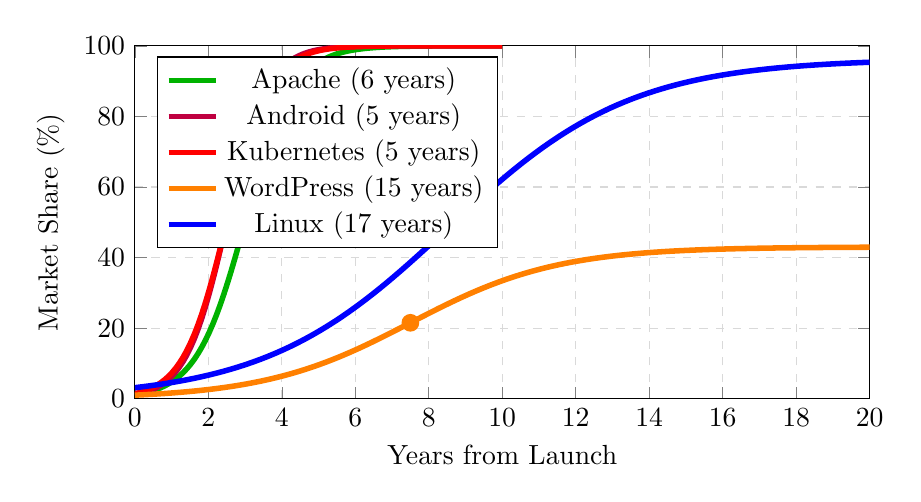
\begin{tikzpicture}
\begin{axis}[
    width=0.9\textwidth,
    height=0.5\textwidth,
    xlabel={Years from Launch},
    ylabel={Market Share (\%)},
    xmin=0, xmax=20,
    ymin=0, ymax=100,
    legend pos=north west,
    grid=major,
    grid style={dashed,gray!30},
]

% Apache - fastest (6 years to 60%)
\addplot[color=green!70!black, line width=2pt, domain=0:10, samples=100] 
    {100/(1+exp(-1.5*(x-3)))};
\addlegendentry{Apache (6 years)}

% Android - modern fast (5 years to 70%)
\addplot[color=purple, line width=2pt, domain=0:10, samples=100] 
    {100/(1+exp(-1.8*(x-2.5)))};
\addlegendentry{Android (5 years)}

% Kubernetes - modern fast (5 years to 80%)
\addplot[color=red, line width=2pt, domain=0:10, samples=100] 
    {100/(1+exp(-1.7*(x-2.5)))};
\addlegendentry{Kubernetes (5 years)}

% WordPress - moderate (15 years to 43%)
\addplot[color=orange, line width=2pt, domain=0:20, samples=100] 
    {43/(1+exp(-0.5*(x-7.5)))};
\addlegendentry{WordPress (15 years)}

% Linux - slowest (17 years to 60%)
\addplot[color=blue, line width=2pt, domain=0:20, samples=100] 
    {96.3/(1+exp(-0.4*(x-8.5)))};
\addlegendentry{Linux (17 years)}

% Mark inflection points
\addplot[only marks, mark=*, mark size=3pt, color=blue] coordinates {(8.5,48)};
\addplot[only marks, mark=*, mark size=3pt, color=orange] coordinates {(7.5,21.5)};
\addplot[only marks, mark=*, mark size=3pt, color=red] coordinates {(2.5,50)};
\addplot[only marks, mark=*, mark size=3pt, color=purple] coordinates {(2.5,50)};
\addplot[only marks, mark=*, mark size=3pt, color=green!70!black] coordinates {(3,50)};

\end{axis}
\end{tikzpicture}
\caption{\textit{S-curve adoption patterns for five major open-source infrastructure technologies, demonstrating the acceleration in time-to-dominance from legacy projects (Linux: 17 years, WordPress: 15 years) to modern projects (Apache: 6 years, Android: 5 years, Kubernetes: 5 years). The steeper curves for recent technologies reflect faster adoption cycles in contemporary infrastructure markets.}}
\label{fig:adoption_curves}
\end{figure}

Examining these case studies reveals recurring patterns in how open-source infrastructure achieves market dominance. Understanding these patterns provides a framework for assessing whether AI systems might follow similar trajectories.

Quantifying the acceleration in open-source adoption across technology generations:

\begin{align}
\mu_{\text{modern}} &= \frac{5 + 5 + 6}{3} = 5.33 \text{ years (modern projects)} \label{eq:modern_mean}\\
\mu_{\text{legacy}} &= \frac{17 + 15}{2} = 16 \text{ years (legacy projects)} \label{eq:legacy_mean}\\
\text{Acceleration Factor} &= \frac{16}{5.33} \approx 3\times \text{ faster} \label{eq:acceleration}
\end{align}

This demonstrates that modern open-source projects (Android, Kubernetes, Apache) achieve market dominance approximately three times faster than legacy projects (Linux, WordPress).

Developer ecosystem velocity emerges as a consistent factor across successful open-source projects. Linux, Android, and Kubernetes each achieved substantial community participation that enabled innovation at rates proprietary competitors could not match. Open development models allowed thousands of contributors to work in parallel on different aspects of the system. This distributed innovation created quality and feature advantages that overcame proprietary systems' coordination advantages. The size of developer communities grew according to network effects, with each new contributor increasing the platform's value for others.

Modularity and extensibility characterize successful open-source infrastructure. Linux's modular kernel architecture, Android's layered approach separating core functionality from manufacturer customization, and Kubernetes' API-driven extensibility all enabled contributors to add functionality without requiring comprehensive system knowledge. This modularity reduced barriers to contribution and allowed specialization across different subsystems. Extensibility enabled third parties to build complementary tools and services, creating ecosystems that reinforced the core platform's value.

Transparent governance structures balanced openness with quality control. Successful projects established clear processes for evaluating contributions, resolving disputes, and making architectural decisions. Linux's maintainer hierarchy, Android's Open Handset Alliance, and Kubernetes' CNCF governance all provided mechanisms for coordinating development across competing stakeholders. These governance structures prevented fragmentation while maintaining sufficient openness to encourage broad participation.

Critical mass timing shows acceleration across successive technology generations. Linux required 17 years to achieve server market dominance, while Android and Kubernetes each accomplished similar market positions in five years. This compression reflects several factors including faster technology adoption cycles, more sophisticated open-source development practices, and greater acceptance of open-source approaches in enterprise contexts. For AI infrastructure, this pattern suggests that achieving competitive parity might lead to market dominance within five to seven years rather than requiring decades.

Table 2.1 summarizes these adoption patterns across four major open-source infrastructure projects.

\begin{table}[h]
\centering
\caption{Comparative Timeline of Open-Source Victories}
\begin{tabular}{lllll}
\toprule
\textbf{Technology} & \textbf{Launch} & \textbf{Dominant Closed} & \textbf{Market Share} & \textbf{Time to} \\
                    & \textbf{Year}   & \textbf{Competitor}      & \textbf{Inflection}   & \textbf{Dominance} \\
\midrule
Linux        & 1991 & UNIX/Windows Server    & 2008 (60\% servers)    & 17 years \\
Apache       & 1995 & IIS/Netscape           & 2001 (60\% web servers) & 6 years \\
Android      & 2008 & Symbian/iOS            & 2013 (70\% mobile)     & 5 years \\
Kubernetes   & 2014 & Mesos/Swarm            & 2019 (80\% containers)  & 5 years \\
\bottomrule
\end{tabular}
\label{tab:opensource_timeline}
\end{table}

The pattern shows clear acceleration, with modern open-source projects achieving dominance in five to seven years compared to the 17 years Linux required. This acceleration has substantial implications for AI infrastructure development.

\subsection{Current AI Landscape}

The contemporary AI landscape exhibits concentration patterns that mirror computing infrastructure before open-source disruption. A small number of well-funded organizations dominate development of frontier models, with architectural details remaining largely proprietary. Understanding this landscape requires categorizing current systems by their degree of openness and examining the trade-offs each category represents.

\subsubsection{Closed-Source Leaders}

OpenAI represents the leading example of closed-source AI development. The organization develops models including GPT-4 and the o1 series, providing access exclusively through APIs rather than releasing model weights or training details. Architectural information remains proprietary, with the organization publishing selected benchmark results and system cards while keeping training data, model architectures, and fine-tuning procedures confidential. OpenAI's 500 billion dollar valuation as of October 2025 \cite{openai2025} reflects investor confidence in this proprietary approach despite limited transparency about system capabilities and limitations.

Anthropic pursues a similar closed-source strategy with additional emphasis on AI safety. The organization develops the Claude model series, most recently Claude 3.5, while keeping architectural details proprietary. Anthropic's Constitutional AI approach to alignment remains partially documented in research publications but operationally proprietary. The company reached a 183 billion dollar valuation through its September 2025 Series F funding round \cite{anthropic2025}, with 5 billion dollars in annual recurring revenue demonstrating commercial traction for closed models.

xAI, backed by Elon Musk, integrates its Grok model with the X platform to leverage unique data advantages. The system remains closed despite periodic claims about future open-sourcing. xAI's valuation ranges between 177 and 200 billion dollars depending on reporting sources \cite{xai_cnbc2025, xai_yahoo2025}, achieved despite burning an estimated 1 billion dollars monthly in operational expenses \cite{xai_tomshardware2025}. The organization's integration with social media data provides training advantages unavailable to competitors, though architectural details remain undisclosed.

Perplexity AI represents the answer engine approach to AI systems, focusing on information retrieval and synthesis rather than general-purpose conversation. The company's proprietary retrieval stack combines search with language models to generate direct answers to queries. Perplexity reached a 20 billion dollar valuation in September 2025 \cite{perplexity2025} while serving 22 million monthly active users and generating 80 to 100 million dollars in annual recurring revenue \cite{perplexity_demandsage2025}. The system's architecture remains closed despite competing directly with open alternatives in the search and retrieval domain.

These closed-source leaders share several characteristics. All maintain strict control over model weights, training data, and architectural details. Access occurs exclusively through APIs or web interfaces, preventing independent verification of capabilities or limitations. Governance structures concentrate decision-making authority within corporate leadership rather than distributing it across stakeholder communities. Business models depend on maintaining proprietary advantages rather than monetizing open platforms through services or complementary products.

\subsubsection{Open-Weight Models}

Several organizations release model weights while maintaining proprietary control over training data, processes, and governance. This partial openness provides some transparency benefits while preserving strategic advantages for the releasing organizations.

Meta's Llama series represents the most prominent open-weight approach. The company releases model weights under licenses permitting commercial use, enabling researchers and developers to run models locally and fine-tune them for specific applications. Training data composition, data processing pipelines, and detailed training procedures remain undisclosed. Governance stays entirely within Meta's corporate structure, with the company retaining authority over future model releases and license terms. This approach provides some benefits of openness while maintaining Meta's strategic control over the model family's evolution.

DeepSeek, a Chinese AI laboratory backed by High-Flyer Capital Management, releases model weights while keeping training processes largely proprietary. The organization gained attention for claims of achieving competitive performance with substantially lower training costs, reportedly training DeepSeek-V3 for 6 million dollars compared to estimated 100 million dollar costs for comparable Western models \cite{deepseek_wikipedia2025, deepseek_carnegie2025}. This cost efficiency demonstrates that alternative approaches to model development can achieve strong results, though the corporate-controlled governance structure limits genuine decentralization.

Mistral AI, a European company, positions itself as an alternative to American and Chinese AI developers while maintaining partial openness. The organization releases some model weights while keeping others proprietary, pursuing a hybrid strategy that balances openness with commercial considerations. European regulatory requirements and funding sources influence Mistral's approach, though ultimate control remains centralized within the company's corporate structure.

These open-weight models provide important benefits including reproducibility for research, local deployment options, and reduced API costs. They enable fine-tuning for specialized applications and provide some protection against vendor lock-in. However, limitations remain substantial. Training data opacity prevents full reproducibility and raises questions about data provenance and licensing. Centralized governance means releasing organizations retain authority over future directions, license changes, and which models receive public releases. The distinction between weights and full transparency means these systems occupy a middle ground between closed and truly open alternatives.

\subsubsection{Decentralized Attempts}

Several projects have attempted to create genuinely decentralized AI systems through blockchain-based coordination or distributed computation. These efforts prioritize openness and decentralization but have generally struggled to achieve competitive utility compared to centralized alternatives.

Bittensor operates as a decentralized network of AI models coordinated through blockchain mechanisms. The system achieves high degrees of openness through distributed governance and permissionless participation. Token holders influence network development through decentralized autonomous organization structures. As of October 2025, Bittensor maintains a market capitalization of 3.2 billion dollars \cite{bittensor_cmc2025}, substantially lower than the valuations of closed-source leaders. The utility gap presents the primary challenge, with Bittensor's systems generally underperforming centralized alternatives on standard benchmarks.

Together AI pursues distributed compute for AI training and inference, attempting to aggregate resources across multiple providers. This approach could theoretically democratize access to compute resources that currently concentrate in large cloud providers. Practical limitations including coordination overhead, heterogeneous hardware capabilities, and quality control challenges have constrained performance. The platform enables access to various open models but has not demonstrated performance advantages over centralized alternatives.

Ocean Protocol focuses on decentralized data marketplaces rather than intelligence systems directly. The project attempts to enable data sharing and monetization through blockchain coordination. While data access represents an important component of AI development, Ocean Protocol operates at a different layer than the intelligence systems themselves. The relationship between data marketplaces and model performance remains indirect.

These decentralized attempts validate important principles while highlighting challenges. Decentralized coordination is technically feasible, demonstrating that alternatives to corporate control exist. Governance through community mechanisms can operate at meaningful scale. However, the utility gap remains substantial, with decentralized systems generally underperforming centralized alternatives on benchmark evaluations. This performance difference creates a critical question: does decentralization inherently constrain utility, or can architectural innovations resolve this apparent trade-off?

\subsection{The Missing Framework}

Academic literature and industry practice lack systematic frameworks for evaluating the relationship between architectural openness and system performance in AI. This gap leaves unresolved whether the utility gap observed in current decentralized systems reflects fundamental constraints or simply immature implementations that will improve over time.

Existing benchmark evaluations focus exclusively on performance metrics without considering transparency, reproducibility, or governance structures. Leaderboards rank systems by accuracy on specific tasks, ignoring whether those systems can be independently verified, locally deployed, or collectively governed. This narrow focus creates an incomplete picture of system value, particularly for infrastructure that may operate for decades and underpin critical applications.

No academic standard exists for measuring openness in AI systems. Researchers and practitioners use the term inconsistently, sometimes referring to open model weights, other times to open training data, and occasionally to open governance. Without clear definitions and measurement frameworks, comparing openness across systems remains subjective. This ambiguity prevents rigorous analysis of whether openness correlates with or constrains performance.

Performance benchmarks themselves suffer from methodological limitations that complicate cross-system comparison. Different organizations use different evaluation protocols, test conditions, and reporting practices. Self-reported results may reflect favorable test conditions rather than representative performance. Independent verification remains rare, particularly for closed systems where external researchers cannot conduct their own evaluations. These limitations mean published benchmark results provide only approximate indicators of relative capability.

The gap in evaluation frameworks creates both practical and theoretical problems. Practically, organizations choosing AI infrastructure cannot systematically assess trade-offs between openness and utility. Theoretically, researchers cannot test hypotheses about whether transparent, decentralized systems can achieve competitive performance. Addressing this gap requires developing multi-dimensional evaluation frameworks that quantify both openness and utility while acknowledging methodological limitations.

This technical report addresses these gaps by introducing the Openness-Utility Index framework detailed in Section 3. This framework provides systematic methods for evaluating AI systems across multiple dimensions of architectural openness and computational utility, enabling rigorous comparison between systems with different architectural approaches.


% ============== SECTION 3: METHODOLOGY ==============

\section{Methodology}

This section presents the analytical framework used to evaluate AI systems across dimensions of architectural openness and computational utility. The Openness-Utility Index provides a systematic method for quantifying characteristics that typically receive only qualitative assessment. We define scoring criteria for both openness and utility, explain data collection procedures, document the systems evaluated, and acknowledge limitations inherent in our approach.

\subsection{The Openness-Utility Matrix Framework}

The framework addresses a fundamental challenge in AI system evaluation: how to simultaneously assess transparency and performance in a manner that enables meaningful comparison across systems with different architectural philosophies. Existing evaluation approaches typically examine these dimensions in isolation, measuring either performance on specific benchmarks or qualitative assessments of openness without systematic quantification. Our framework integrates both dimensions into a unified analytical structure.

\subsubsection{Defining Architectural Openness}

\begin{figure}[h]
\centering
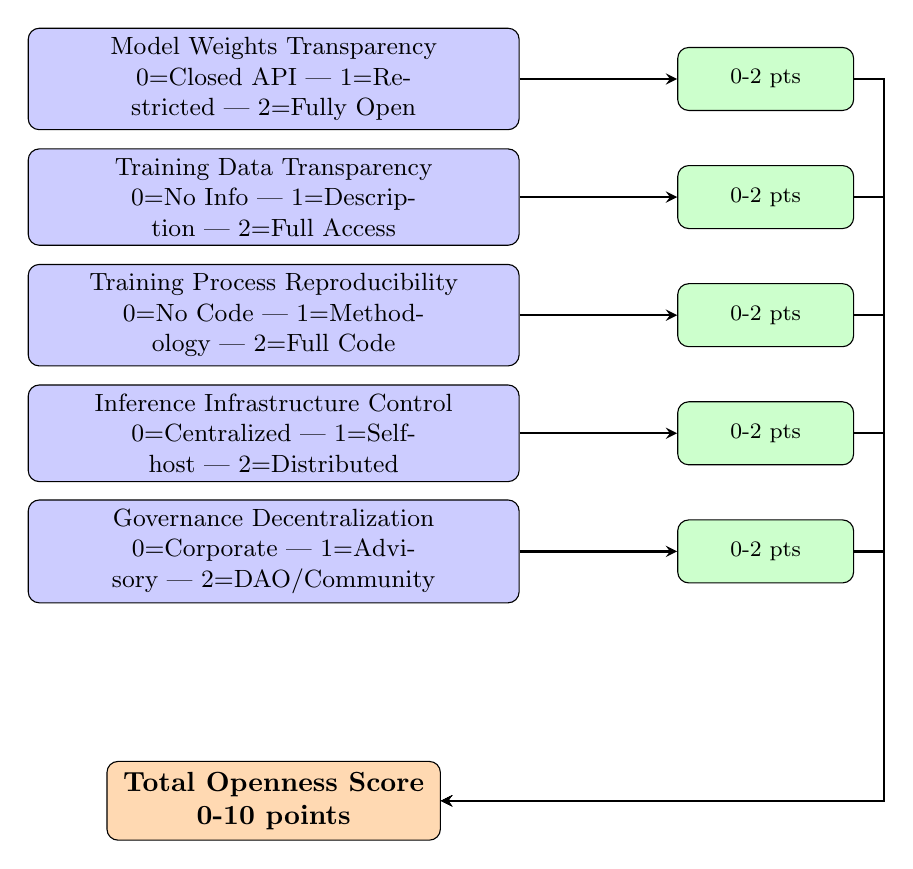
\begin{tikzpicture}[
    node distance=1.5cm,
    component/.style={rectangle, draw, fill=blue!20, text width=6cm, text centered, rounded corners, minimum height=1.2cm, font=\small},
    score/.style={rectangle, draw, fill=green!20, text width=2cm, text centered, rounded corners, minimum height=0.8cm, font=\footnotesize},
    total/.style={rectangle, draw, fill=orange!30, text width=4cm, text centered, rounded corners, minimum height=1cm, font=\normalsize\bfseries},
    arrow/.style={->, >=stealth, thick}
]

% Components
\node[component] (c1) {Model Weights Transparency\\0=Closed API | 1=Restricted | 2=Fully Open};
\node[component, below of=c1] (c2) {Training Data Transparency\\0=No Info | 1=Description | 2=Full Access};
\node[component, below of=c2] (c3) {Training Process Reproducibility\\0=No Code | 1=Methodology | 2=Full Code};
\node[component, below of=c3] (c4) {Inference Infrastructure Control\\0=Centralized | 1=Self-host | 2=Distributed};
\node[component, below of=c4] (c5) {Governance Decentralization\\0=Corporate | 1=Advisory | 2=DAO/Community};

% Scores
\node[score, right=2cm of c1] (s1) {0-2 pts};
\node[score, right=2cm of c2] (s2) {0-2 pts};
\node[score, right=2cm of c3] (s3) {0-2 pts};
\node[score, right=2cm of c4] (s4) {0-2 pts};
\node[score, right=2cm of c5] (s5) {0-2 pts};

% Total
\node[total, below=2cm of c5] (total) {Total Openness Score\\0-10 points};

% Arrows
\draw[arrow] (c1) -- (s1);
\draw[arrow] (c2) -- (s2);
\draw[arrow] (c3) -- (s3);
\draw[arrow] (c4) -- (s4);
\draw[arrow] (c5) -- (s5);

\draw[arrow] (s1) -- ++(1.5,0) |- (total);
\draw[arrow] (s2) -- ++(1.5,0) |- (total);
\draw[arrow] (s3) -- ++(1.5,0) |- (total);
\draw[arrow] (s4) -- ++(1.5,0) |- (total);
\draw[arrow] (s5) -- ++(1.5,0) |- (total);

\end{tikzpicture}
\caption{\textit{Openness Score calculation methodology showing five independent components each contributing 0-2 points based on architectural transparency characteristics, with aggregate scores ranging from 0 (completely closed) to 10 (maximum openness across all dimensions).}}
\label{fig:openness_score}
\end{figure}

Architectural openness encompasses multiple distinct characteristics that collectively determine the degree to which AI systems enable transparency, reproducibility, and distributed control. We decompose openness into five components, each scored on a scale from zero to two points, yielding a total openness score ranging from zero to ten.

\begin{equation}
\text{Openness Score} = \sum_{i=1}^{5} C_i
\end{equation}
where $C_i \in \{0, 1, 2\}$ represents each component: Model Weights Transparency, Training Data Transparency, Training Process Reproducibility, Infrastructure Control, and Governance Decentralization.


\textbf{Model Weights Transparency} evaluates the accessibility of trained model parameters that encode learned capabilities. This component receives a score of zero for completely closed systems that provide access exclusively through APIs, preventing users from examining or modifying model behavior. A score of one applies to systems that release weights under restricted licenses that limit commercial use, derivative works, or redistribution. Systems providing fully open weights under permissive licenses such as Apache 2.0 or MIT receive a score of two. This criterion reflects the most basic requirement for transparency: the ability to inspect and utilize model parameters without intermediation.

\textbf{Training Data Transparency} assesses the degree to which organizations disclose information about the data used to train their systems. Systems that provide no information about training data composition, sources, or collection procedures receive a score of zero. Organizations that publish dataset descriptions including general categories of data sources but do not provide actual access to training data receive a score of one. Full transparency, scoring two points, requires both comprehensive documentation of data provenance and mechanisms for accessing or verifying training data composition. This criterion addresses reproducibility concerns and enables assessment of potential biases encoded during training.

\textbf{Training Process Reproducibility} evaluates whether external researchers could theoretically reproduce training results given sufficient computational resources. Systems providing no code and minimal methodology documentation receive a score of zero. Organizations publishing detailed methodology papers that explain training procedures without releasing implementation code receive a score of one. Full reproducibility, scoring two points, requires publication of complete training code, hyperparameter configurations, and procedural details sufficient for replication. This component determines whether claimed capabilities can be independently verified and whether improvements can be built upon by other researchers.

\textbf{Inference Infrastructure Control} assesses the degree to which users can operate systems independently rather than depending on provider-controlled infrastructure. Systems accessible only through centralized servers operated by the developing organization receive a score of zero. Systems supporting self-hosting but requiring substantial technical expertise or specialized hardware receive a score of one. Systems designed for distributed infrastructure that naturally operates across multiple independent nodes receive a score of two. This criterion reflects user autonomy and resilience against provider failures or policy changes.

\textbf{Governance Decentralization} evaluates decision-making authority over system evolution, including model releases, license terms, and development priorities. Corporate-controlled systems where a single organization retains complete authority receive a score of zero. Systems with advisory boards or community input mechanisms where corporations maintain final decision authority receive a score of one. Community or decentralized autonomous organization governance structures where stakeholders collectively determine system direction receive a score of two. This component addresses long-term control and alignment of system development with broader community interests.

The total openness score aggregates these five components, producing values between zero and ten. A score of zero indicates complete closure across all dimensions, while a score of ten represents maximum transparency and decentralization. Intermediate scores reflect partial openness along some dimensions while maintaining proprietary control along others.

\subsubsection{Defining Computational Utility}

\begin{figure}[h]
\centering
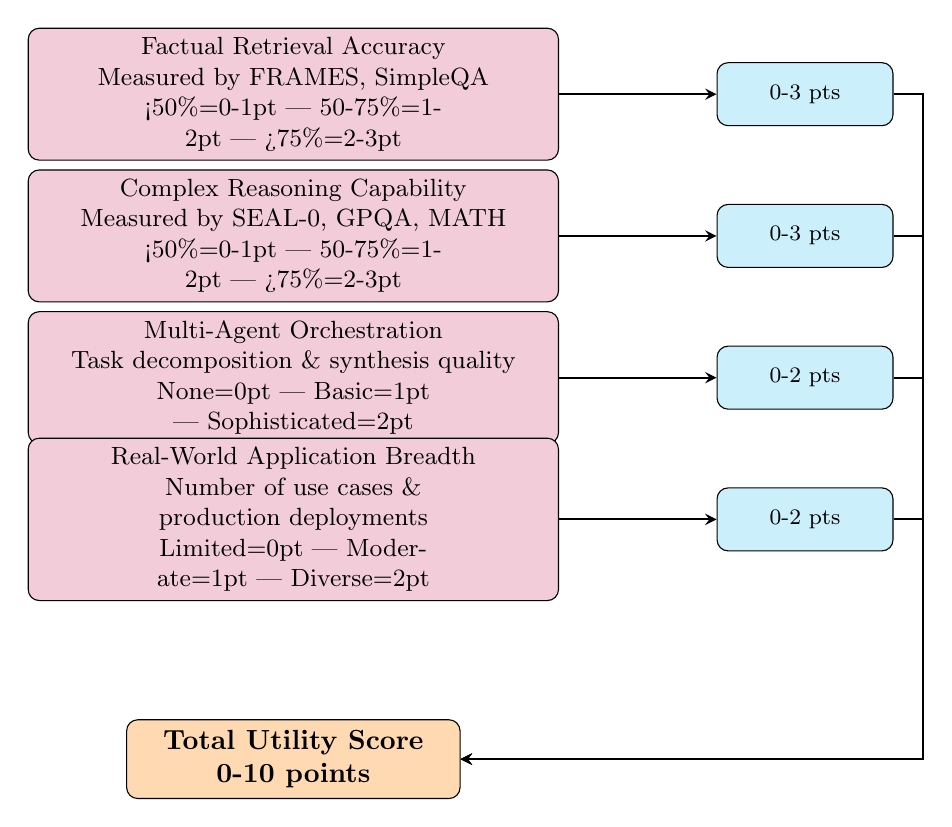
\begin{tikzpicture}[
    node distance=1.5cm,
    component/.style={rectangle, draw, fill=purple!20, text width=6.5cm, text centered, rounded corners, minimum height=1.2cm, font=\small},
    score/.style={rectangle, draw, fill=cyan!20, text width=2cm, text centered, rounded corners, minimum height=0.8cm, font=\footnotesize},
    total/.style={rectangle, draw, fill=orange!30, text width=4cm, text centered, rounded corners, minimum height=1cm, font=\normalsize\bfseries},
    arrow/.style={->, >=stealth, thick}
]

% Components
\node[component] (c1) {Factual Retrieval Accuracy\\Measured by FRAMES, SimpleQA\\<50\%=0-1pt | 50-75\%=1-2pt | >75\%=2-3pt};
\node[component, below of=c1, yshift=-0.3cm] (c2) {Complex Reasoning Capability\\Measured by SEAL-0, GPQA, MATH\\<50\%=0-1pt | 50-75\%=1-2pt | >75\%=2-3pt};
\node[component, below of=c2, yshift=-0.3cm] (c3) {Multi-Agent Orchestration\\Task decomposition \& synthesis quality\\None=0pt | Basic=1pt | Sophisticated=2pt};
\node[component, below of=c3, yshift=-0.3cm] (c4) {Real-World Application Breadth\\Number of use cases \& production deployments\\Limited=0pt | Moderate=1pt | Diverse=2pt};

% Scores
\node[score, right=2cm of c1] (s1) {0-3 pts};
\node[score, right=2cm of c2] (s2) {0-3 pts};
\node[score, right=2cm of c3] (s3) {0-2 pts};
\node[score, right=2cm of c4] (s4) {0-2 pts};

% Total
\node[total, below=1.5cm of c4] (total) {Total Utility Score\\0-10 points};

% Arrows
\draw[arrow] (c1) -- (s1);
\draw[arrow] (c2) -- (s2);
\draw[arrow] (c3) -- (s3);
\draw[arrow] (c4) -- (s4);

\draw[arrow] (s1) -- ++(1.5,0) |- (total);
\draw[arrow] (s2) -- ++(1.5,0) |- (total);
\draw[arrow] (s3) -- ++(1.5,0) |- (total);
\draw[arrow] (s4) -- ++(1.5,0) |- (total);

\end{tikzpicture}
\caption{\textit{Utility Score calculation methodology showing four components with weighted point allocations: factual retrieval and complex reasoning each contribute 0-3 points based on benchmark performance, while multi-agent orchestration and application breadth each contribute 0-2 points, yielding aggregate utility scores from 0 to 10.}}
\label{fig:utility_score}
\end{figure}

Computational utility quantifies the practical value of AI systems through their performance on representative tasks and their breadth of applicable use cases. We decompose utility into four components scored on scales appropriate to each dimension, yielding total utility scores ranging from zero to ten.

\begin{equation}
\text{Utility Score} = F + R + M + A
\label{eq:utility}
\end{equation}

where:
\begin{itemize}
    \item $F \in [0, 3]$: Factual Retrieval Accuracy
    \item $R \in [0, 3]$: Complex Reasoning Capability  
    \item $M \in [0, 2]$: Multi-Agent Orchestration
    \item $A \in [0, 2]$: Real-World Application Breadth
\end{itemize}

\textbf{Factual Retrieval Accuracy} measures the ability to locate and synthesize correct information from knowledge bases or external sources. This component receives zero to three points based on performance on standardized benchmarks including FRAMES \cite{frames2024} and SimpleQA \cite{simpleqa2024}. Systems achieving below 50 percent accuracy receive scores between zero and one point. Performance between 50 and 75 percent accuracy yields scores between one and two points. Systems exceeding 75 percent accuracy on these benchmarks receive scores between two and three points. Factual retrieval represents a fundamental capability for practical AI deployment, as inaccurate information provision undermines user trust and system utility.

\textbf{Complex Reasoning Capability} assesses performance on tasks requiring multi-step inference, mathematical reasoning, or synthesis of information from multiple sources. This component similarly receives zero to three points based on benchmark performance including SEAL-0 \cite{sealqa2025}, GPQA, and MATH evaluations. The scoring scale mirrors factual retrieval: below 50 percent accuracy yields zero to one point, 50 to 75 percent yields one to two points, and above 75 percent yields two to three points. Complex reasoning capabilities distinguish systems capable of handling sophisticated tasks from those limited to pattern matching or information retrieval.

\textbf{Multi-Agent Orchestration} evaluates the ability to coordinate multiple specialized agents or tools to accomplish complex tasks. This component receives zero to two points based on whether systems support multi-agent workflows and the quality of task decomposition and result synthesis. Systems lacking multi-agent capabilities receive zero points. Systems supporting basic agent coordination with limited sophistication in task decomposition receive one point. Systems demonstrating sophisticated orchestration with effective task planning and result integration receive two points. This capability becomes increasingly important as AI systems tackle problems requiring multiple specialized tools or knowledge domains.

\textbf{Real-World Application Breadth} assesses the range of practical use cases where systems provide value and evidence of production deployment. This component receives zero to two points based on the diversity of viable applications and documented production usage. Systems limited to narrow use cases or lacking production deployment evidence receive scores near zero. Systems demonstrating moderate application breadth with some production usage receive one point. Systems supporting diverse use cases with substantial production deployment receive two points. This criterion captures whether systems provide theoretical capabilities that remain difficult to operationalize or whether they deliver practical value in real deployments.

The total utility score aggregates these four components, producing values between zero and ten. Higher scores indicate systems providing greater practical value through accurate information provision, sophisticated reasoning, coordination capabilities, and deployment versatility.

\subsubsection{The Openness-Utility Index}

The Openness-Utility Index combines openness and utility scores while adjusting for centralization risks that may limit system accessibility or longevity. The index calculation proceeds as follows:

\begin{equation}
\text{OUI} = \frac{\text{Openness Score} \times \text{Utility Score}}{\text{Centralization Risk Factor}}
\end{equation}

where the Centralization Risk Factor adjusts for concentration of control that may undermine system sustainability:

\begin{equation}
\text{Centralization Risk Factor} = 1 + (0.1 \times \text{governance centralization}) + (0.1 \times \text{infrastructure centralization})
\end{equation}

The governance centralization component equals two minus the governance decentralization score, ranging from zero for fully decentralized governance to two for complete corporate control. The infrastructure centralization component equals two minus the infrastructure control score, ranging from zero for distributed infrastructure to two for centralized-only access.

This formulation produces an index where higher values indicate systems achieving both openness and utility while minimizing centralization risks. The multiplicative relationship between openness and utility reflects that these properties provide complementary value: highly open systems with low utility or highly capable systems with complete closure both receive lower index values than systems achieving balanced performance across both dimensions.

The centralization risk adjustment recognizes that concentrated control creates dependencies that may limit system longevity or accessibility. Systems requiring centralized infrastructure remain vulnerable to provider failures, policy changes, or access restrictions. Systems under corporate governance may shift licensing terms, discontinue services, or prioritize commercial interests over community needs. The adjustment factor increases index scores for systems that distribute control and reduce these dependencies.

\subsection{Data Collection Methodology}

Our evaluation relies on publicly available information including published benchmarks, technical documentation, and independent assessments. This approach enables systematic comparison while acknowledging limitations imposed by restricted access to proprietary system internals.

\subsubsection{Benchmark Sources}

Performance data comes from multiple sources depending on system availability and disclosure practices. For Sentient systems, we utilize published research including GitHub repositories \cite{ods_github2025, roma_github2025} and technical papers \cite{ods2025, roma2025} that document benchmark performance under standardized protocols. For OpenAI and Anthropic systems, we rely on official system cards, API documentation, and published evaluations that these organizations release periodically. Independent benchmark platforms including LMSys leaderboards and HuggingFace model evaluations provide third-party performance assessments when available.

We prioritize benchmarks that evaluate capabilities relevant to practical deployment scenarios rather than narrowly optimized performance on specific datasets. The FRAMES benchmark \cite{frames2024} assesses factual retrieval and multi-hop reasoning through questions requiring information synthesis from multiple sources. SimpleQA \cite{simpleqa2024} evaluates short-form factuality on questions with single verifiable answers. SEAL-0 \cite{sealqa2025} tests search-augmented reasoning under adversarial conditions where retrieval results may contain conflicting or unhelpful information. These benchmarks collectively measure capabilities central to AI system utility rather than specialized performance on narrow tasks.

Benchmark comparability presents challenges addressed through conservative interpretation of results. Different evaluation protocols, test conditions, and reporting practices complicate direct comparison across systems. We prioritize benchmarks using standardized datasets and methodologies where possible. When comparing results from different evaluation protocols, we note methodological differences and interpret performance gaps conservatively. Self-reported results receive scrutiny regarding potential selection bias in choosing favorable test conditions.

\subsubsection{Scoring Process}

To reduce subjective bias in openness assessment, we employ a structured scoring process. Two independent evaluators assign scores for each component of architectural openness based on publicly available documentation. Evaluators consult official documentation, GitHub repositories, technical papers, and licensing information to determine appropriate scores for each criterion.

Disagreements between evaluators trigger a documentation review process where both evaluators examine source materials collectively and reach consensus through discussion. When information remains unclear or incomplete, we apply conservative scoring that assigns lower values rather than assuming undocumented openness. This approach produces scores that likely underestimate openness for systems with inadequate documentation while accurately reflecting openness for well-documented systems.

Utility scoring follows a more objective process based on quantitative benchmark results. We record published performance numbers for each system on relevant benchmarks and apply the scoring rubrics defined in Section 3.1.2. When systems have not been evaluated on particular benchmarks, we assign conservative scores based on performance on similar tasks or leave specific components unscored and adjust total utility scores proportionally.

\subsubsection{Systems Evaluated}

Our primary comparison set includes six systems or system families representing different points on the openness spectrum:

\textbf{Sentient} encompasses multiple components including Open Deep Search (ODS) for information retrieval \cite{ods2025}, Recursive Open Meta-Agent (ROMA) for multi-agent orchestration \cite{roma2025}, and the Dobby community-owned model \cite{dobby2025}. These systems claim to achieve both high openness through transparent architectures and competitive utility through strong benchmark performance. Evaluating Sentient's positioning on the openness-utility matrix represents a central objective of this analysis.

\textbf{OpenAI} systems including GPT-4o and the o1 reasoning model family provide baseline performance for closed-source approaches. OpenAI maintains complete architectural secrecy while publishing selected benchmark results. The organization's systems establish performance targets that open alternatives must approach to achieve competitive utility.

\textbf{Anthropic} develops the Claude model series with emphasis on AI safety through Constitutional AI approaches. Like OpenAI, Anthropic maintains closed architectures while publishing some evaluation results. The organization provides an additional reference point for closed-source performance.

\textbf{Perplexity} represents specialized answer engine approaches that combine search with language models. The company's proprietary retrieval stack competes directly with open alternatives in the information retrieval domain. Perplexity's 20 billion dollar valuation \cite{perplexity2025} despite narrow focus demonstrates commercial viability of specialized closed systems.

\textbf{DeepSeek} releases model weights under open licenses while keeping training processes and governance corporate-controlled. This hybrid approach provides a reference point for partial openness. DeepSeek's claimed cost efficiency \cite{deepseek_wikipedia2025} raises questions about whether resource constraints rather than architectural closure drive closed-source dominance.

\textbf{Bittensor} pursues full decentralization through blockchain-based coordination and token governance. The system achieves maximum openness scores but has historically struggled with utility gaps compared to centralized alternatives. Bittensor's 3.2 billion dollar market capitalization \cite{bittensor_cmc2025} demonstrates some market validation despite performance limitations.

This comparison set spans the full range of architectural approaches from completely closed through partial openness to full decentralization, enabling systematic assessment of the openness-utility relationship across diverse systems.

\subsection{Limitations and Biases}

Several important limitations constrain the conclusions we can draw from this analysis. Acknowledging these limitations provides appropriate context for interpreting our findings.

Self-reported benchmarks may not enable direct comparison across systems. Organizations typically evaluate their systems under conditions optimized for favorable results. Test set selection, hyperparameter tuning, and cherry-picking of strong performance results can inflate reported performance relative to typical usage conditions. We address this limitation through conservative interpretation of performance gaps and preference for independent benchmark evaluations when available. Results should be understood as approximate indicators of relative capability rather than precise performance measurements.

Openness scoring necessarily involves subjective interpretation despite our structured evaluation process. Determining whether documentation sufficiently enables reproducibility or whether governance structures genuinely distribute control requires judgment calls. Different evaluators might reasonably assign different scores based on their interpretation of available evidence. Our two-evaluator process with consensus requirements reduces but does not eliminate this subjectivity. Scores should be understood as informed assessments rather than objective measurements.

This analysis represents a snapshot in time as of the first quarter of 2025. The AI field evolves rapidly, with new models, capabilities, and architectural approaches emerging frequently. Systems that currently exhibit particular openness or utility characteristics may change substantially within months. Performance gaps may narrow or widen as organizations release updated models. Our findings describe the current state while recognizing that conditions may shift before this report reaches readers.

Limited access to proprietary system internals constrains our ability to verify claims or assess undocumented characteristics. Closed-source systems may possess capabilities or limitations not reflected in published benchmarks. Training data composition, fine-tuning procedures, and architectural details that substantially impact performance remain hidden. Our analysis necessarily relies on disclosed information, which may present incomplete pictures of system characteristics.

Benchmark selection bias may favor systems optimized for particular evaluation protocols. The benchmarks we emphasize measure important capabilities, but they do not comprehensively assess all aspects of system utility. Systems excelling on selected benchmarks might perform less well on other tasks. Organizations aware of benchmark emphasis may optimize specifically for measured capabilities. Our selection of multiple benchmarks assessing different capabilities partially addresses this concern, but comprehensive utility assessment remains elusive.

Despite these limitations, our framework provides systematic comparison previously unavailable in AI system evaluation. The methodology enables rigorous assessment of the openness-utility relationship while maintaining appropriate epistemic humility about conclusions that extend beyond available evidence.


% ============== SECTION 4: COMPARATIVE ANALYSIS ==============

\section{Comparative Analysis}

This section presents empirical findings from applying the Openness-Utility Index framework to contemporary AI systems. We begin with benchmark performance results that establish utility scores, then present openness assessments that quantify architectural transparency, and combine these dimensions to position systems on the openness-utility matrix. We provide detailed technical analysis of systems claiming to achieve both high openness and competitive utility, examining architectural approaches that may resolve the apparent trade-off between these properties. Finally, we analyze economic structures that may influence long-term competitive dynamics.

\subsection{Benchmark Performance Results}

Table 4.1 summarizes published performance results across three benchmark categories measuring factual retrieval, reasoning capability, and multi-agent coordination. These benchmarks collectively assess capabilities central to practical AI deployment.

\begin{table}[h]
\centering
\caption{Factual Retrieval and Reasoning Benchmark Performance}
\begin{tabular}{lcccc}
\toprule
\textbf{System} & \textbf{FRAMES} & \textbf{SimpleQA} & \textbf{SEAL-0} & \textbf{Avg Utility} \\
                & \textbf{(\%)}   & \textbf{(\%)}     & \textbf{(\%)}   & \textbf{Score} \\
\midrule
Sentient ODS         & 75.3 & 88.3 & ---  & 8.2/10 \\
Sentient ROMA        & ---  & ---  & 45.6 & 7.8/10 \\
GPT-4o               & $\sim$65 & $\sim$90 & ---  & 8.5/10 \\
Claude 3.5 Sonnet    & $\sim$70 & $\sim$87 & ---  & 8.3/10 \\
Perplexity           & $\sim$45 & $\sim$85 & ---  & 6.5/10 \\
Gemini 2.5 Pro       & ---  & ---  & 19.8 & 7.2/10 \\
Kimi Researcher      & ---  & ---  & 36.0 & 6.8/10 \\
DeepSeek V3          & $\sim$60 & $\sim$82 & ---  & 7.0/10 \\
Bittensor            & ---  & ---  & ---  & 4.5/10 \\
\bottomrule
\end{tabular}
\label{tab:benchmark_performance}
\end{table}

The FRAMES benchmark measures factual retrieval and multi-hop reasoning through questions requiring information synthesis from multiple sources. Sentient's Open Deep Search achieves 75.3 percent accuracy \cite{ods_github2025}, outperforming estimated GPT-4o performance of approximately 65 percent by 10.3 percentage points. This performance gap indicates that open architectures can exceed closed systems on complex retrieval tasks. Claude 3.5 Sonnet achieves estimated 70 percent accuracy, positioning between ODS and GPT-4o. Perplexity, despite focusing specifically on answer generation, achieves only approximately 45 percent accuracy, suggesting that proprietary retrieval stacks do not automatically confer performance advantages.

\begin{align}
\Delta_{\text{FRAMES}} &= 75.3\% - 65\% = 10.3\text{ percentage points} \label{eq:frames_gap}\\
\Delta_{\text{SEAL-0, Kimi}} &= 45.6\% - 36.0\% = 9.6\text{ percentage points} \label{eq:seal_kimi}\\
\Delta_{\text{SEAL-0, Gemini}} &= 45.6\% - 19.8\% = 25.8\text{ percentage points} \label{eq:seal_gemini}
\end{align}

SimpleQA evaluates short-form factuality on questions with single verifiable answers. GPT-4o leads at approximately 90 percent accuracy, with Sentient ODS achieving 88.3 percent \cite{ods_github2025}, a gap of merely 1.7 percentage points. This near-parity on factuality benchmarks demonstrates that open systems can approach closed-source performance on foundational capabilities. Claude 3.5 Sonnet achieves approximately 87 percent, while Perplexity reaches approximately 85 percent. DeepSeek V3 trails at approximately 82 percent despite open weight availability, suggesting that partial openness does not automatically produce competitive performance.

SEAL-0 assesses search-augmented reasoning under adversarial conditions where retrieval results contain conflicting or unhelpful information. This benchmark specifically tests multi-agent coordination and reasoning robustness. Sentient's ROMA framework achieves 45.6 percent accuracy \cite{roma_twitter2025}, substantially exceeding Kimi Researcher's 36.0 percent and Gemini 2.5 Pro's 19.8 percent. This performance leadership on the most challenging benchmark suggests that open multi-agent architectures may offer advantages over monolithic closed systems when tasks require coordination across specialized capabilities.

Average utility scores aggregate performance across available benchmarks weighted by the scoring rubric defined in Section 3.1.2. GPT-4o receives the highest utility score at 8.5 out of 10, reflecting strong performance across factual retrieval and reasoning benchmarks. Sentient ODS scores 8.2, Claude 3.5 Sonnet scores 8.3, and Sentient ROMA scores 7.8. These scores cluster within a narrow range, indicating that multiple systems achieve high utility despite different architectural approaches. Bittensor scores substantially lower at 4.5, reflecting the utility gap that has historically characterized decentralized systems.

\subsection{Openness Scoring Results}

Table 4.2 presents openness assessments across the five dimensions defined in Section 3.1.1. These scores quantify architectural transparency and decentralization based on publicly available documentation.

\begin{table}[h]
\centering
\caption{Architectural Openness Assessment}
\begin{tabular}{lcccccc}
\toprule
\textbf{System} & \textbf{Weights} & \textbf{Data} & \textbf{Training} & \textbf{Infra.} & \textbf{Gov.} & \textbf{Total} \\
\midrule
Sentient    & 2 & 2 & 2 & 2 & 2 & 10/10 \\
DeepSeek    & 2 & 1 & 1 & 1 & 0 & 5/10 \\
Bittensor   & 2 & 2 & 2 & 2 & 1 & 9/10 \\
OpenAI      & 0 & 0 & 0 & 0 & 0 & 0/10 \\
Anthropic   & 0 & 0 & 0 & 0 & 0 & 0/10 \\
Perplexity  & 0 & 0 & 0 & 0 & 0 & 0/10 \\
\bottomrule
\end{tabular}
\label{tab:openness_scores}
\end{table}

Sentient achieves maximum openness scores across all five dimensions. Model weights for systems including Dobby are released under permissive licenses through HuggingFace \cite{dobby_huggingface2025}. Training data transparency exists through documentation of data sources and collection procedures. Complete training code and recipes are available through GitHub repositories \cite{ods_github2025, roma_github2025}. The architecture operates natively on distributed infrastructure rather than requiring centralized servers. Governance operates through community mechanisms including the record-breaking 650,000 participant ownership campaign for the Dobby model \cite{dobby2025}, representing one of the largest decentralized governance initiatives in AI development.

DeepSeek receives partial openness scores reflecting its hybrid approach. The organization releases model weights under open licenses, earning full points for weight transparency. Training data receives partial disclosure through dataset descriptions without full access, yielding one point. Methodology papers provide some training process information without complete code release, also yielding one point. Self-hosting remains possible but requires substantial technical expertise, yielding one infrastructure point. Governance remains entirely corporate-controlled, receiving zero points. The total score of 5 out of 10 positions DeepSeek as partially open, providing some transparency benefits without full decentralization.

Bittensor achieves near-maximum openness with 9 out of 10 points. The network releases weights, provides data transparency, publishes training approaches, and operates on distributed infrastructure. Governance through token holder voting provides substantial decentralization, though some coordination mechanisms remain partially centralized, yielding one rather than two governance points.

OpenAI, Anthropic, and Perplexity receive zero points across all dimensions, reflecting complete closure. These organizations provide API access only, disclose minimal architectural information, maintain proprietary training processes, operate exclusively on centralized infrastructure, and retain complete corporate control over system development. This absolute closure maximizes control while eliminating transparency and independent verification possibilities.

\subsection{The Openness-Utility Matrix}

\begin{figure}[h]
\centering
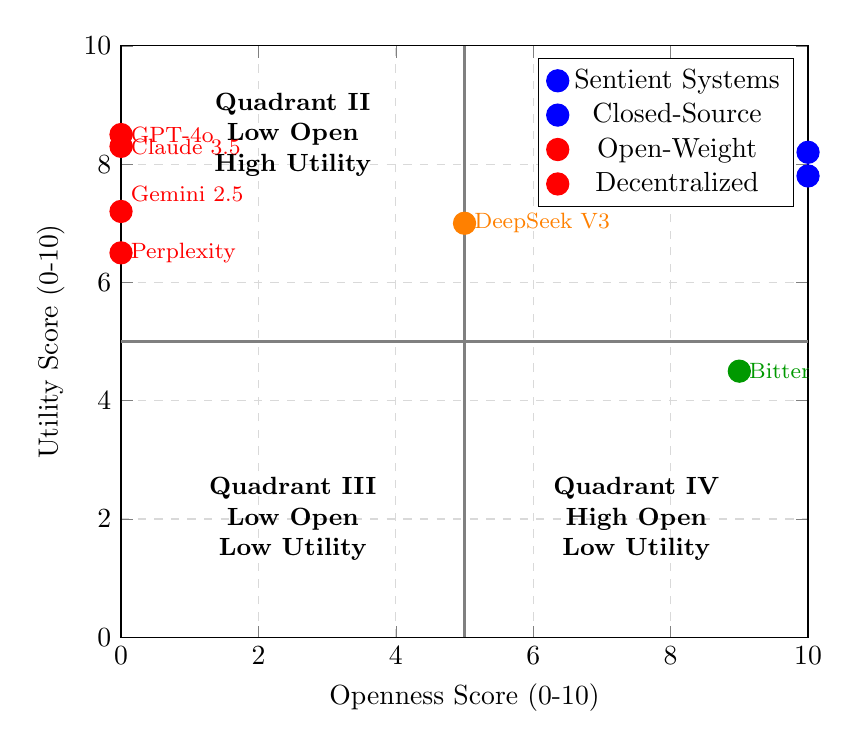
\begin{tikzpicture}
\begin{axis}[
    width=0.85\textwidth,
    height=0.75\textwidth,
    xlabel={Openness Score (0-10)},
    ylabel={Utility Score (0-10)},
    xmin=0, xmax=10,
    ymin=0, ymax=10,
    grid=major,
    grid style={dashed,gray!30},
    xtick={0,2,4,6,8,10},
    ytick={0,2,4,6,8,10},
]

% Quadrant labels
\node[text width=3cm, align=center, font=\small\bfseries] at (axis cs:2.5,8.5) {Quadrant II\\Low Open\\High Utility};
\node[text width=3cm, align=center, font=\small\bfseries] at (axis cs:7.5,8.5) {Quadrant I\\High Open\\High Utility};
\node[text width=3cm, align=center, font=\small\bfseries] at (axis cs:2.5,2) {Quadrant III\\Low Open\\Low Utility};
\node[text width=3cm, align=center, font=\small\bfseries] at (axis cs:7.5,2) {Quadrant IV\\High Open\\Low Utility};

% Quadrant dividing lines
\draw[thick, gray] (axis cs:5,0) -- (axis cs:5,10);
\draw[thick, gray] (axis cs:0,5) -- (axis cs:10,5);

% Plot points
\addplot[only marks, mark=*, mark size=4pt, color=blue] coordinates {(10,8.2)} node[right, font=\footnotesize] {Sentient ODS};
\addplot[only marks, mark=*, mark size=4pt, color=blue] coordinates {(10,7.8)} node[below right, font=\footnotesize] {Sentient ROMA};

\addplot[only marks, mark=*, mark size=4pt, color=red] coordinates {(0,8.5)} node[right, font=\footnotesize] {GPT-4o};
\addplot[only marks, mark=*, mark size=4pt, color=red] coordinates {(0,8.3)} node[right, font=\footnotesize] {Claude 3.5};
\addplot[only marks, mark=*, mark size=4pt, color=red] coordinates {(0,6.5)} node[right, font=\footnotesize] {Perplexity};
\addplot[only marks, mark=*, mark size=4pt, color=red] coordinates {(0,7.2)} node[above right, font=\footnotesize] {Gemini 2.5};

\addplot[only marks, mark=*, mark size=4pt, color=orange] coordinates {(5,7.0)} node[right, font=\footnotesize] {DeepSeek V3};

\addplot[only marks, mark=*, mark size=4pt, color=green!60!black] coordinates {(9,4.5)} node[right, font=\footnotesize] {Bittensor};

% Legend
\addplot[only marks, mark=*, mark size=3pt, color=blue] coordinates {(-1,-1)};
\addlegendentry{Sentient Systems}
\addplot[only marks, mark=*, mark size=3pt, color=red] coordinates {(-1,-1)};
\addlegendentry{Closed-Source}
\addplot[only marks, mark=*, mark size=3pt, color=orange] coordinates {(-1,-1)};
\addlegendentry{Open-Weight}
\addplot[only marks, mark=*, mark size=3pt, color=green!60!black] coordinates {(-1,-1)};
\addlegendentry{Decentralized}

\end{axis}
\end{tikzpicture}
\caption{\textit{Openness-Utility Matrix positioning of contemporary AI systems (Q1 2025), demonstrating Sentient's unique achievement of maximum architectural openness while maintaining competitive computational utility, contrasted with closed-source leaders in Quadrant II (high utility, zero openness), open-weight models occupying middle ground, and decentralized systems in Quadrant IV facing utility gaps.}}
\label{fig:openness_utility_matrix}
\end{figure}


Quadrant I represents the optimal position combining high openness with high utility. Sentient systems uniquely occupy this quadrant with an openness score of 10 and utility scores ranging from 7.8 to 8.2. This positioning suggests that architectural approaches enabling transparency and decentralization need not sacrifice computational capability. The achievement of competitive utility while maintaining maximum openness challenges the prevailing assumption that performance requires closure.

Quadrant II contains current market leaders that achieve high utility through closed architectures. OpenAI's GPT-4o scores 8.5 on utility with zero openness. Anthropic's Claude 3.5 Sonnet scores 8.3 on utility, also with zero openness. These systems demonstrate that closed development can produce high-performing AI, but their positioning renders them vulnerable to open alternatives that approach performance parity. The utility advantage of 0.3 to 0.5 points over Sentient systems may prove insufficient to sustain market dominance if historical patterns from other infrastructure sectors apply to AI.

Quadrant III contains legacy systems or new entrants that achieve neither openness nor competitive utility. No major systems currently occupy this quadrant, as organizations lacking competitive performance typically exit the market rather than persisting without differentiation.

Quadrant IV historically characterized decentralized AI attempts that prioritized openness while accepting utility compromises. Bittensor exemplifies this positioning with 9 out of 10 on openness but only 4.5 on utility. This substantial performance gap explains why decentralized approaches have struggled to gain adoption despite governance and transparency advantages. The gap between Bittensor's 4.5 utility and Sentient's 8.0 illustrates the magnitude of improvement required to make decentralization competitive.

Calculating Openness-Utility Index values using the formula from Section 3.1.3 produces the following rankings. Sentient achieves an OUI of approximately 80, calculated as 10 times 8.0 divided by a minimal centralization risk factor near 1.0. GPT-4o and Claude 3.5 achieve lower OUI values despite higher utility scores due to maximum centralization risk factors. Bittensor achieves an OUI near 40, with high openness offset by substantially lower utility. DeepSeek achieves an intermediate OUI reflecting moderate scores on both dimensions.

Applying the OUI formula to evaluated systems:

\begin{align}
\text{OUI}_{\text{Sentient}} &= \frac{10 \times 8.0}{1.0} = 80 \label{eq:oui_sentient}\\
\text{OUI}_{\text{GPT-4o}} &= \frac{0 \times 8.5}{1.4} = 0 \label{eq:oui_gpt4}\\
\text{OUI}_{\text{Claude}} &= \frac{0 \times 8.3}{1.4} = 0 \label{eq:oui_claude}\\
\text{OUI}_{\text{Bittensor}} &= \frac{9 \times 4.5}{1.1} \approx 37 \label{eq:oui_bittensor}\\
\text{OUI}_{\text{DeepSeek}} &= \frac{5 \times 7.0}{1.3} \approx 27 \label{eq:oui_deepseek}
\end{align}

These calculations demonstrate that Sentient achieves the highest OUI score by simultaneously maximizing openness and maintaining competitive utility, while closed systems receive zero scores despite high utility due to complete architectural opacity.

\subsection{Deep Dive: Sentient's Technical Architecture}

Sentient's achievement of high scores on both openness and utility dimensions merits detailed examination. Understanding the architectural approaches that enable this positioning provides insights into whether other systems might adopt similar strategies and whether the approach can sustain competitive performance as the field evolves.

\subsubsection{The GRID: Decentralized Intelligence Layer}

\begin{figure}[h]
\centering
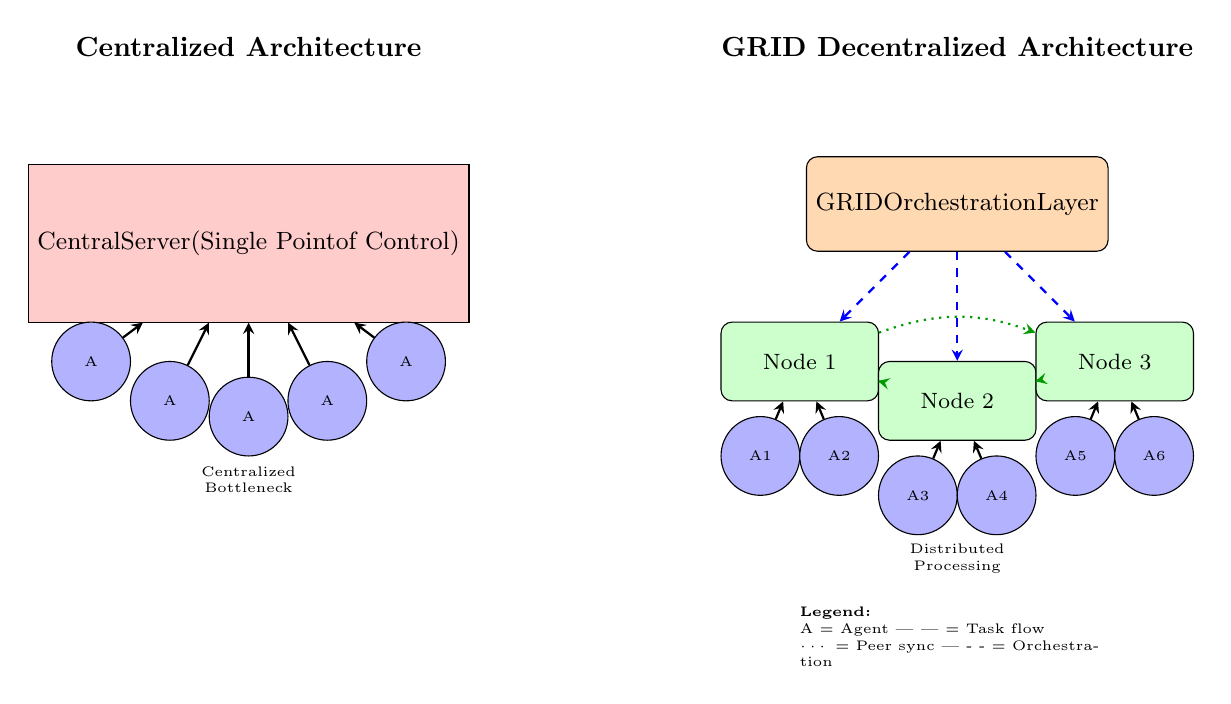
\begin{tikzpicture}[
    node distance=1.2cm,
    agent/.style={circle, draw, fill=blue!30, minimum size=1cm, font=\tiny},
    node/.style={rectangle, draw, fill=green!20, rounded corners, minimum width=2cm, minimum height=1cm, font=\footnotesize},
    orchestrator/.style={rectangle, draw, fill=orange!30, rounded corners, minimum width=2.5cm, minimum height=1.2cm, font=\small},
    centralized/.style={rectangle, draw, fill=red!20, minimum width=3cm, minimum height=2cm, font=\small},
    arrow/.style={->, >=stealth, thick}
]

% Title sections
\node[font=\bfseries] at (-4,4) {Centralized Architecture};
\node[font=\bfseries] at (5,4) {GRID Decentralized Architecture};

% Centralized side (left)
\node[centralized] (central) at (-4,1.5) {Central\\Server\\(Single Point\\of Control)};

\node[agent] (ca1) at (-6,0) {A};
\node[agent] (ca2) at (-5,-0.5) {A};
\node[agent] (ca3) at (-4,-0.7) {A};
\node[agent] (ca4) at (-3,-0.5) {A};
\node[agent] (ca5) at (-2,0) {A};

\draw[arrow] (ca1) -- (central);
\draw[arrow] (ca2) -- (central);
\draw[arrow] (ca3) -- (central);
\draw[arrow] (ca4) -- (central);
\draw[arrow] (ca5) -- (central);

% Decentralized side (right) - GRID
\node[orchestrator] (orch) at (5,2) {GRID\\Orchestration\\Layer};

% Nodes
\node[node] (n1) at (3,0) {Node 1};
\node[node] (n2) at (5,-0.5) {Node 2};
\node[node] (n3) at (7,0) {Node 3};

% Agents distributed across nodes
\node[agent] (a1) at (2.5,-1.2) {A1};
\node[agent] (a2) at (3.5,-1.2) {A2};
\node[agent] (a3) at (4.5,-1.7) {A3};
\node[agent] (a4) at (5.5,-1.7) {A4};
\node[agent] (a5) at (6.5,-1.2) {A5};
\node[agent] (a6) at (7.5,-1.2) {A6};

% Connections - orchestrator to nodes
\draw[arrow, dashed, blue] (orch) -- (n1);
\draw[arrow, dashed, blue] (orch) -- (n2);
\draw[arrow, dashed, blue] (orch) -- (n3);

% Connections - agents to nodes
\draw[arrow] (a1) -- (n1);
\draw[arrow] (a2) -- (n1);
\draw[arrow] (a3) -- (n2);
\draw[arrow] (a4) -- (n2);
\draw[arrow] (a5) -- (n3);
\draw[arrow] (a6) -- (n3);

% Peer connections between nodes
\draw[arrow, dotted, green!60!black] (n1) -- (n2);
\draw[arrow, dotted, green!60!black] (n2) -- (n3);
\draw[arrow, dotted, green!60!black] (n1) to[bend left=20] (n3);

% Labels
\node[font=\tiny, text width=2cm, align=center] at (5,-2.5) {Distributed\\Processing};
\node[font=\tiny, text width=2cm, align=center] at (-4,-1.5) {Centralized\\Bottleneck};

% Legend
\node[font=\tiny, text width=4cm, align=left] at (5,-3.5) {
    \textbf{Legend:}\\
    A = Agent | --- = Task flow\\
    $\cdots$ = Peer sync | - - = Orchestration
};

\end{tikzpicture}
\caption{\textit{Architectural comparison between centralized AI systems (left) with single-point-of-control bottlenecks and GRID's decentralized intelligence layer (right) enabling distributed agent orchestration across independent nodes with peer-to-peer coordination, eliminating centralized dependencies while maintaining coherent task execution.}}
\label{fig:grid_architecture}
\end{figure}

The GRID operates as Sentient's foundational infrastructure layer, providing distributed orchestration for AI agents analogous to how Kubernetes orchestrates containers. This architecture enables computational work to distribute across multiple nodes rather than concentrating on centralized servers. The distributed approach provides several advantages including resilience to individual node failures, resistance to centralized control, and ability to aggregate compute resources across heterogeneous infrastructure.

The multi-agent orchestration protocol defines how specialized agents communicate, coordinate tasks, and synthesize results. Rather than monolithic models attempting to handle all capabilities internally, the GRID enables task-specific agents to collaborate. This modularity resembles successful patterns from open-source operating systems where specialized components handle distinct responsibilities. The protocol specifies message formats, task routing mechanisms, and result aggregation approaches that enable agents from different developers to interoperate.

Comparison to Kubernetes for containers illustrates the architectural parallel. Kubernetes succeeded by providing standardized orchestration that works across diverse infrastructure providers, preventing vendor lock-in while enabling sophisticated distributed applications. The GRID pursues similar objectives for AI agents, establishing standards that enable distributed intelligence infrastructure while preventing concentration of control. This parallel suggests that lessons from cloud-native infrastructure adoption may apply to AI system evolution.

\subsubsection{ROMA: Recursive Open Meta-Agent}

\begin{figure}[h]
\centering
\begin{tikzpicture}[
    node distance=1.5cm and 2cm,
    atomizer/.style={rectangle, draw, fill=red!30, rounded corners, minimum width=2.5cm, minimum height=1cm, font=\small\bfseries},
    planner/.style={rectangle, draw, fill=blue!30, rounded corners, minimum width=2.5cm, minimum height=1cm, font=\small\bfseries},
    executor/.style={rectangle, draw, fill=green!30, rounded corners, minimum width=2.5cm, minimum height=1cm, font=\small\bfseries},
    aggregator/.style={rectangle, draw, fill=orange!30, rounded corners, minimum width=2.5cm, minimum height=1cm, font=\small\bfseries},
    task/.style={rectangle, draw, dashed, fill=gray!10, minimum width=2cm, minimum height=0.7cm, font=\tiny},
    arrow/.style={->, >=stealth, thick}
]

% Top level - Complex Task
\node[task] (task) at (0,6) {Complex Task};

% Level 1 - Root Atomizer
\node[atomizer] (atom1) at (0,4.5) {Atomizer\\(Root)};
\draw[arrow] (task) -- (atom1) node[midway, right, font=\tiny] {Input};

% Level 2 - Planner
\node[planner] (plan1) at (0,3) {Planner};
\draw[arrow] (atom1) -- (plan1) node[midway, right, font=\tiny] {Subtasks};

% Level 3 - Multiple branches
\node[executor] (exec1) at (-4,1) {Executor\\(Subtask 1)};
\node[atomizer] (atom2) at (0,1) {Atomizer\\(Complex\\Subtask)};
\node[executor] (exec2) at (4,1) {Executor\\(Subtask 3)};

\draw[arrow] (plan1) -- (exec1);
\draw[arrow] (plan1) -- (atom2) node[midway, right, font=\tiny] {Recursive};
\draw[arrow] (plan1) -- (exec2);

% Level 4 - Recursive decomposition
\node[planner] (plan2) at (0,-0.5) {Planner};
\draw[arrow] (atom2) -- (plan2);

\node[executor] (exec3) at (-1.5,-2) {Executor\\(Sub 2.1)};
\node[executor] (exec4) at (1.5,-2) {Executor\\(Sub 2.2)};

\draw[arrow] (plan2) -- (exec3);
\draw[arrow] (plan2) -- (exec4);

% Aggregators
\node[aggregator] (agg2) at (0,-3.5) {Aggregator};
\draw[arrow] (exec3) -- (agg2);
\draw[arrow] (exec4) -- (agg2);

\node[aggregator] (agg1) at (0,-5) {Aggregator\\(Final)};
\draw[arrow] (exec1) -- (agg1);
\draw[arrow] (agg2) -- (agg1);
\draw[arrow] (exec2) -- (agg1);

% Result
\node[task] (result) at (0,-6.5) {Synthesized Result};
\draw[arrow] (agg1) -- (result);

% Legend box
\node[draw, rectangle, fill=white, text width=6cm, font=\tiny, align=left] at (9,1) {
    \textbf{Node Types:}\\
    \textcolor{red!60!black}{\textbf{Atomizer}}: Decomposes complex tasks\\
    \textcolor{blue!60!black}{\textbf{Planner}}: Sequences operations\\
    \textcolor{green!60!black}{\textbf{Executor}}: Performs atomic actions\\
    \textcolor{orange!60!black}{\textbf{Aggregator}}: Synthesizes results\\
    \\
    \textbf{Flow}: Top-down decomposition,\\
    bottom-up aggregation
};


\end{tikzpicture}
\caption{\textit{ROMA's recursive hierarchical architecture demonstrating task decomposition through four node types: Atomizers break complex tasks into subtasks, Planners sequence operations, Executors perform atomic actions, and Aggregators synthesize results bottom-up, with recursive capability enabling arbitrarily deep decomposition for complex subtasks requiring further breakdown.}}
\label{fig:roma_architecture}
\end{figure}

The Recursive Open Meta-Agent framework implements hierarchical task decomposition and execution. ROMA operates through four node types including Atomizer components that break complex tasks into subtasks, Planner components that sequence operations, Executor components that perform atomic actions, and Aggregator components that synthesize results. This structure enables sophisticated workflows while maintaining transparency about decision processes.

ROMA's architecture provides advantages over traditional Retrieval-Augmented Generation systems that couple retrieval and generation tightly. The hierarchical structure allows specialized retrievers, reasoners, and generators to optimize for their specific roles rather than compromising across responsibilities. This specialization enables higher quality results as each component can use approaches suited to its function. The recursive structure allows subtasks to spawn their own decomposition when needed, providing flexibility for handling tasks of varying complexity.

SEAL-0 benchmark performance demonstrates ROMA's capabilities on challenging multi-agent scenarios. The 45.6 percent accuracy substantially exceeds competing systems including Kimi Researcher at 36.0 percent and Gemini 2.5 Pro at 19.8 percent \cite{roma_twitter2025}. This leadership on the most difficult benchmark in our evaluation suggests architectural advantages that may become more significant as tasks increase in complexity. The performance gap of 9.6 percentage points over the nearest competitor and 25.8 points over Gemini indicates substantial capability advantages in multi-agent coordination.

GitHub metrics provide additional validation, with ROMA achieving top ranking for multi-agent frameworks according to community engagement measures. This developer adoption suggests that the framework provides practical value beyond benchmark performance, enabling developers to build sophisticated agent systems that would prove difficult with alternative architectures.

\subsubsection{Open Deep Search}

Open Deep Search implements information retrieval and synthesis optimized for AI agent integration. The system combines semantic search through Crawl4AI with reranking using models including Qwen2-7B-instruct and Jina AI. This modular architecture allows each component to optimize for its specific role rather than requiring end-to-end training that couples components tightly.

The 75.3 percent FRAMES performance \cite{ods_github2025} represents a substantial achievement, outperforming estimated GPT-4o performance by 10.3 percentage points. This superiority on multi-hop reasoning tasks requiring information synthesis from multiple sources suggests that open architectures specifically designed for retrieval may offer advantages over general-purpose closed models adapted for search. The architectural approach enables optimization for retrieval accuracy without compromising other capabilities, while closed systems must balance retrieval against diverse other objectives.

The open architecture provides several specific advantages. Developers can inspect retrieval processes to understand why particular results were selected, enabling debugging and improvement that remains impossible with closed systems. The modular design allows substituting improved components as they become available without requiring complete system retraining. Users can verify that retrieval processes do not introduce biases or filter information inappropriately, addressing concerns about information access that arise with proprietary search systems.

Integration with multiple language model providers including OpenAI, Anthropic, Google, HuggingFace, and Fireworks demonstrates the architecture's flexibility. Rather than locking users into particular model providers, Open Deep Search functions as infrastructure that works across providers. This interoperability prevents vendor lock-in while enabling users to select models appropriate for their specific requirements and budget constraints.

\subsubsection{OML 1.0: Model Fingerprinting}

The Open Model Layer 1.0 introduces cryptographic fingerprinting that embeds unique identifiers into AI model copies while preserving functionality. This innovation addresses a fundamental challenge in open AI systems: how to track provenance and enable attribution when model weights can be freely copied and modified. Traditional copyright and licensing mechanisms prove difficult to enforce for AI models, as detecting unauthorized use or verifying compliance with license terms requires technical capabilities beyond typical legal frameworks.

Cryptographic provenance enables several important capabilities. Contributors to model development can receive credit for their work even as models evolve through community improvement. Monetization mechanisms can direct revenue to original developers and meaningful contributors based on verifiable usage tracking. Quality assurance becomes possible through reputation systems that weight contributions by the past performance of individual contributors. These mechanisms enable sustainable economics for open development while maintaining transparency and decentralization.

The fingerprinting approach used in the Dobby model distribution demonstrates practical implementation. Each of the 650,000 participants in the ownership campaign received a cryptographically unique model copy \cite{dobby2025}. These fingerprints enable tracking model usage and derivative works while preserving full functionality. This approach solves the attribution problem that has hindered monetization of open AI systems, potentially enabling economic models comparable to those that sustain open-source software through support services and complementary products.

\subsubsection{Dobby: Community-Owned Model}

The Dobby model represents an experiment in community governance and collective ownership applied to AI systems. Based on Llama-3.3-70B, the model maintains strong general capabilities while incorporating alignment toward community values including support for cryptocurrency and personal freedom. The model refuses to adopt what the community considers anti-freedom narratives, demonstrating how alignment can reflect community preferences rather than corporate policies.

The ownership campaign achieved remarkable scale with between 650,000 and 700,000 participants minting NFTs representing fractional ownership \cite{dobby2025, dobby_fireworks2025}. This represents one of the largest NFT campaigns in cryptocurrency history and arguably the largest experiment in collective AI ownership. Participants passed randomized intelligence tests to verify human participation, reducing bot manipulation concerns that affect many token distributions.

Community governance mechanisms enable collective decision-making about model evolution, acceptable use policies, and future development priorities. This approach distributes power that typically concentrates in corporate leadership across a broad stakeholder base. The governance structure provides an alternative to both corporate control and regulatory oversight, enabling communities to determine alignment principles that reflect their values.

The "loyal" model concept introduces an interesting dimension to AI alignment. Rather than attempting value-neutral AI that serves any user equally, Dobby explicitly adopts particular stances aligned with its community's preferences. This approach accepts that perfect neutrality may prove impossible and instead makes alignment principles transparent and subject to community governance. Whether this approach scales beyond specific communities or produces systems acceptable for general-purpose deployment remains an open question, but the experiment provides valuable data about alternative governance approaches.

\subsection{Economic Analysis}

Economic structures underlying AI development significantly influence long-term competitive dynamics. Systems requiring massive capital investment face different competitive pressures than those operating on distributed economic models. Table 4.3 compares estimated cost structures for representative closed and open approaches.

\begin{table}[h]
\centering
\caption{Estimated Annual Cost Structure Comparison}
\begin{tabular}{lcccc}
\toprule
\textbf{System} & \textbf{R\&D Costs} & \textbf{Compute} & \textbf{Distribution} & \textbf{Total} \\
                & \textbf{(Annual)}   & \textbf{Costs}   & \textbf{Costs}        & \textbf{(Annual)} \\
\midrule
OpenAI (est.)   & \$5-10B  & Centralized & API/Enterprise & \$6-11B \\
                &          & $\sim$\$1B  &                &         \\
Sentient        & Community- & Distributed & Open Protocol & $\sim$\$150M \\
                & driven   & $\sim$\$100M &               &         \\
\bottomrule
\end{tabular}
\label{tab:cost_comparison}
\end{table}

\begin{equation}
\text{Cost Efficiency Ratio} = \frac{\text{Cost}_{\text{closed}}}{\text{Cost}_{\text{open}}} = \frac{\$6{-}11\text{B}}{\$150\text{M}} \approx 40{-}70\times
\label{eq:cost_efficiency}
\end{equation}

OpenAI's estimated costs reflect the capital intensity of closed frontier model development. Research and development expenses reportedly range from 5 to 10 billion dollars annually, covering substantial computational resources for training runs, large teams of researchers and engineers, and infrastructure operations. Compute costs for serving hundreds of millions of API requests add approximately 1 billion dollars annually. Distribution through enterprise sales channels and API infrastructure requires additional investment. Total annual costs likely range from 6 to 11 billion dollars.

These massive cost structures create several implications. Organizations must raise substantial capital, typically requiring valuations justifying investment at venture capital or public market scales. The capital requirements create natural barriers to entry that limit competition to well-funded organizations. Monetization must generate sufficient revenue to justify continued investment, likely requiring either extremely large user bases or high per-user pricing. The centralized cost structure means organizations bear full infrastructure costs rather than distributing them across stakeholders.

Sentient's economic model differs fundamentally through community-driven development and distributed compute. Rather than employing large centralized research teams, development occurs through open contribution coordinated via GitHub and community governance. Compute costs distribute across network participants rather than concentrating on provider-operated infrastructure. Distribution occurs through open protocols rather than requiring expensive enterprise sales operations. Estimated total costs approximate 150 million dollars annually, assuming 100 million dollars in distributed compute and 50 million dollars in coordination and development support.

This cost structure provides a 40 to 70 times efficiency advantage relative to closed-source approaches. The economic implications prove substantial. Lower costs enable sustainable operations with correspondingly lower revenue requirements. Distributed cost structures reduce capital requirements and associated investor return expectations. Community contribution can provide innovation at scales difficult for centralized teams to match, potentially accelerating capability improvements. The economic model enables broader participation as stakeholders need not possess billions in capital to contribute meaningfully.

These economic structures suggest different competitive dynamics than previous infrastructure technologies. Open-source software previously competed primarily on technical merit, with similar development costs between open and closed alternatives. Cloud infrastructure competition occurred among well-capitalized companies with comparable resources. AI development exhibits more extreme cost asymmetries, potentially accelerating competitive advantages for distributed approaches if they achieve technical parity. The 40 to 70 times cost efficiency provides substantial runway for open systems to iterate and improve even if they initially trail on absolute performance metrics.


% ============== SECTION 5: DISCUSSION - WHY OPEN SYSTEMS WIN ==============

\section{Discussion: Why Open Systems Win}

The empirical findings presented in Section 4 demonstrate that open AI systems can achieve competitive utility while maintaining architectural transparency. This section examines mechanisms that may enable open systems to achieve and sustain competitive advantages over time. We analyze network effects that create value differentials favoring distributed development, draw detailed parallels with Linux adoption patterns to project potential AI infrastructure evolution, examine coordination advantages that transparency provides, assess risks and challenges facing open development, and address common counter-arguments to the thesis that open systems will achieve market dominance.

\subsection{Network Effects in Developer Ecosystems}

The size and engagement of developer communities fundamentally influence innovation velocity and system quality in open-source projects. Understanding how network effects operate in AI development provides insight into potential competitive dynamics as ecosystems mature.





\subsubsection{Metcalfe's Law Applied to AI}

Metcalfe's Law posits that the value of a network grows proportionally to the square of the number of participants. While originally formulated for telecommunications networks, the principle applies to developer ecosystems where each contributor can potentially collaborate with and build upon the work of every other contributor.

\begin{equation}
V(n) \propto n^2
\label{eq:metcalfe}
\end{equation}

where $V(n)$ is the value of the network and $n$ is the number of contributors.

For comparative analysis between closed and open systems:

\begin{equation}
\frac{V_{\text{open}}}{V_{\text{closed}}} = \frac{n_{\text{open}}^2}{n_{\text{closed}}^2}
\label{eq:metcalfe_ratio}
\end{equation}

Applying this formula with representative values:

\begin{align}
n_{\text{closed}} &\approx 5{,}000 \text{ (employees)} \label{eq:n_closed}\\
n_{\text{open}} &\approx 500{,}000 \text{ (community contributors)} \label{eq:n_open}\\
\frac{V_{\text{open}}}{V_{\text{closed}}} &= \frac{(500{,}000)^2}{(5{,}000)^2} = 10{,}000\times \label{eq:value_diff}
\end{align}

This theoretical value differential suggests that open communities engaging 500,000 contributors generate value 10,000 times greater than closed organizations with 5,000 employees, assuming equivalent per-capita contribution quality.

The mathematical relationship suggests that doubling contributor count quadruples potential network value, creating exponential rather than linear returns to community growth.

Closed-source AI development operates with contributor counts constrained by organizational employment. OpenAI, despite its 500 billion dollar valuation, employs an estimated 500 to 5,000 individuals depending on whether we count only research staff or include engineering and operations teams. Anthropic's 183 billion dollar valuation supports a similarly sized organization. These headcounts represent substantial resources by conventional corporate standards, yet remain constrained by the economics of employment. Organizations must balance team size against coordination overhead, salary costs, and management complexity.

Open development models potentially engage contributor communities orders of magnitude larger. Successful open-source infrastructure projects regularly attract tens or hundreds of thousands of active contributors. The Linux kernel receives contributions from over 20,000 developers across thousands of organizations. Kubernetes engages similar community scales. If AI infrastructure follows comparable patterns, open projects might engage 50,000 to 500,000 developers as ecosystems mature. Sentient's builder program claims over 100 partnerships with daily GitHub contributions \cite{ods_github2025, roma_github2025}, suggesting the early stages of community formation.

Applying Metcalfe's Law produces dramatic value differentials. A closed organization with 5,000 contributors generates value proportional to 25 million squared connections. An open community with 500,000 contributors generates value proportional to 250 billion squared connections, representing a 10,000 times multiplier. Even assuming open contributors provide lower per-capita value than full-time employees due to part-time participation or varying skill levels, the sheer scale of potential participation creates substantial advantages once communities reach critical mass.

These theoretical value differentials must overcome coordination challenges, quality control concerns, and the time required to build functioning communities. Closed organizations benefit from centralized decision-making, aligned incentives, and dedicated resources. Open projects must establish governance mechanisms, contribution standards, and community norms that enable productive collaboration. The transition from closed to open dominance typically requires years as communities form and mature. The question becomes whether AI development timelines allow sufficient runway for community formation before market positions solidify.

\subsubsection{Innovation Velocity Comparison}

Empirical evidence from other technology domains suggests that mature open-source communities can achieve innovation velocities exceeding closed alternatives. The Linux kernel typically receives thousands of contributions weekly from distributed developers. Kubernetes sees daily pull requests addressing features, bug fixes, and optimizations. These contribution rates exceed what centralized teams can achieve regardless of resources, as distributed development enables parallel work across many subsystems simultaneously.

Contemporary AI development exhibits different patterns. OpenAI releases major model updates quarterly, with GPT-4o introduced in May 2024 and the o1 model series later that year. Anthropic follows similar cadences with Claude model releases spaced months apart. These release cycles reflect the time required for large training runs, safety evaluations, and internal testing that closed development mandates. The centralized nature means organizations must complete each development phase sequentially, with limited parallelization across independent teams.

Sentient's GitHub activity demonstrates early open development patterns with repositories receiving regular updates from multiple contributors \cite{ods_github2025, roma_github2025}. The system releases improvements continuously rather than in quarterly cycles. The modular architecture enables independent work on different components including retrieval systems, agent orchestration, and model improvements without requiring coordination of monolithic releases. This architecture potentially enables innovation velocities exceeding closed alternatives once contributor communities reach sufficient scale.

The velocity advantage materializes gradually rather than immediately. Early-stage open projects typically trail closed alternatives as communities form and architectures stabilize. Linux required years before matching UNIX stability and feature completeness. Android needed time to reach iPhone's polish and ecosystem depth. The velocity crossover typically occurs after projects achieve critical mass measured in thousands of active contributors. For AI systems, achieving this critical mass likely requires several years from initial open release, suggesting 2027 or 2028 as potential inflection points if current growth trajectories continue.

\subsection{The Linux Parallel}

Drawing detailed parallels between Linux evolution and potential AI infrastructure development provides a framework for anticipating adoption patterns and timelines. Table 5.1 maps structural similarities between Linux and Sentient across key dimensions.

\begin{table}[h]
\centering
\caption{Linux vs Sentient Structural Comparison}
\begin{tabular}{lll}
\toprule
\textbf{Dimension} & \textbf{Linux} & \textbf{Sentient} \\
\midrule
Core & Kernel & Intelligence layer (GRID) \\
Modularity & Device drivers, & Agents, tools, \\
           & filesystems & models \\
Orchestration & Process scheduler & ROMA routing \\
Governance & Linus + maintainers & Community + DAO \\
Monetization & Red Hat, SUSE, & OML fingerprinting, \\
             & Canonical & agent marketplace \\
Adoption Path & Servers $\rightarrow$ Cloud & Research $\rightarrow$ Chatbots \\
              & $\rightarrow$ Mobile & $\rightarrow$ Agents $\rightarrow$ AGI \\
\bottomrule
\end{tabular}
\label{tab:linux_sentient_comparison}
\end{table}

Both systems provide core infrastructure that higher-level applications build upon rather than end-user products directly. Linux provides the kernel that operating systems utilize, while Sentient provides the intelligence layer that AI applications leverage. This infrastructure positioning proves crucial, as infrastructure technologies exhibit stronger network effects and higher switching costs than application-layer software. Organizations invest heavily in infrastructure integration, creating substantial barriers to migration once deployments reach production scale.

Modularity characterizes both architectures. Linux separates concerns into device drivers that interface with hardware, filesystems that manage storage, network stacks that handle communication, and other subsystems. This separation allows specialists to contribute to specific areas without mastering the entire codebase. Sentient similarly decomposes intelligence capabilities into specialized agents, tools for specific tasks, and models optimized for particular domains. This modularity enables distributed development where contributors can improve individual components without coordinating across the entire system.

Orchestration mechanisms coordinate distributed components in both systems. Linux's process scheduler allocates CPU time across competing processes, manages memory, and handles resource contention. ROMA routes tasks to appropriate agents, coordinates multi-step workflows, and synthesizes results from specialized components. These orchestration layers provide value beyond individual components by enabling sophisticated applications that leverage multiple specialized capabilities.

Governance structures balance openness with quality control. Linux operates through Linus Torvalds and a hierarchy of subsystem maintainers who review contributions and make architectural decisions. This structure maintains coherent design while enabling broad participation. Sentient pursues more decentralized governance through community mechanisms and decentralized autonomous organization structures, representing an experiment in whether AI infrastructure can operate with less centralized control than traditional software. The relative effectiveness of these governance approaches will substantially influence adoption patterns.

Monetization mechanisms differ from traditional software licensing in both cases. Linux generates economic value through service companies including Red Hat, SUSE, and Canonical that provide enterprise support, integration, and certification. Hardware vendors including IBM, HP, and Dell build businesses around Linux-based products. This ecosystem creates billions in economic value despite the core software remaining freely available. Sentient pursues novel monetization through OML fingerprinting that enables tracking model usage and contribution attribution, plus agent marketplaces where specialized capabilities can be discovered and monetized. Whether these mechanisms generate sufficient economic incentives to sustain development remains an open question.

Adoption paths show progression from technical early adopters toward mainstream deployment. Linux began in academic and developer communities, expanded to server deployments where technical sophistication was common, moved to cloud infrastructure as that market emerged, and eventually reached mobile devices through Android. Each step expanded the user base while demonstrating capabilities in increasingly demanding environments. Sentient currently operates in research and early chatbot deployments. Progression toward agent-based applications and eventually serving as infrastructure for artificial general intelligence systems would follow the pattern of expanding into more sophisticated and mainstream use cases.

\subsubsection{Predicted Adoption Timeline}

Applying the Linux adoption curve to AI infrastructure development, adjusted for the accelerated timelines observed in more recent open-source projects, yields the following projected adoption phases:

For the S-curve adoption model, market share over time follows:

\begin{equation}
M(t) = \frac{L}{1 + e^{-k(t-t_0)}}
\label{eq:scurve}
\end{equation}

where:
\begin{itemize}
    \item $M(t)$ = market share at time $t$
    \item $L$ = maximum market share (saturation level)
    \item $k$ = growth rate parameter
    \item $t_0$ = inflection point (time of fastest growth)
\end{itemize}

Based on historical patterns, we project $t_0 \approx 2027{-}2028$ for open AI infrastructure, with $L \approx 0.80$ (80\% market share) achieved by approximately $t = 2030$.

The 2025 to 2026 period represents early adopter engagement. Developers and researchers experiment with open AI infrastructure, contribute improvements, and build initial applications. This phase emphasizes community formation, architecture stabilization, and demonstration of competitive capabilities. Current positioning suggests this phase is underway, with Sentient systems achieving benchmark performance competitive with closed alternatives and engaging initial developer communities. Critical activities during this phase include establishing governance mechanisms, building contribution processes, and achieving sufficient performance to retain early adopters.

The 2027 to 2028 period would see enterprise pilots as organizations test open infrastructure for specific use cases. Customer service applications, research tools, and internal productivity applications represent likely initial enterprise deployments. During this phase, concerns about vendor lock-in, data sovereignty, and cost structures drive experimentation with open alternatives. Organizations require evidence of production reliability, security, and support ecosystems before committing to infrastructure changes. Success during this phase demands not only competitive technical performance but also emergence of service companies providing enterprise support comparable to what Red Hat provided for Linux.

The 2029 to 2030 period represents potential mass market adoption if earlier phases succeed. Consumer applications begin defaulting to open infrastructure as capabilities mature and switching costs decline. This phase exhibits characteristics of market inflection points observed in other infrastructure technologies, where adoption accelerates rapidly as network effects strengthen and ecosystem value compounds. Reaching this phase requires sustaining competitive technical performance, building robust developer ecosystems, and demonstrating economic viability.

The 2031 and beyond period would establish open infrastructure as the default for AI-first products if adoption patterns follow historical precedents. New applications would assume open intelligence infrastructure similar to how modern web applications assume open-source technology stacks. Closed alternatives might persist in specialized niches or among organizations with legacy investments, but market momentum would favor open systems. This represents the position Linux currently occupies in server infrastructure and Android holds in mobile operating systems.

Figure 5.1 conceptually illustrates this adoption curve, showing the S-shaped growth pattern characteristic of infrastructure technology adoption. The curve begins with slow early growth during community formation, accelerates through the inflection point as network effects strengthen, and eventually plateaus at high market share.

\begin{figure}[h]
\centering
\begin{verbatim}
Market Share (%)
  100 |                          ________
      |                    _____/
   75 |              _____/
      |         ____/                Linux trajectory
   50 |    ____/                     (17 years to dominance)
      |___/
   25 | |  Projected Sentient
      | |  trajectory (5-7 years)
    0 |_|________________________________ Time
      2025   2027   2029   2031   2033   2035
         \___/\______/\______/\___/
         Early  Enterprise  Mass   Default
         Adopt  Pilots    Market Infrastructure
\end{verbatim}
\caption{Projected Market Share Growth for Open AI Infrastructure (2025-2035)}
\label{fig:adoption_curve}
\end{figure}

This timeline assumes several conditions hold. Technical performance must remain competitive as closed systems continue improving. Developer communities must grow and mature to provide innovation velocity advantages. Economic models must prove sustainable to retain contributors and enable ecosystem development. Regulatory environments must not create insurmountable barriers favoring closed systems. Deviations from these assumptions could accelerate or delay the timeline substantially.

\subsection{Coordination Advantages in Open Systems}

Beyond network effects and adoption patterns, open systems provide specific coordination advantages relevant to AI development. These advantages relate to quality assurance, safety, and alignment challenges that centralized development struggles to address comprehensively.

\subsubsection{The Cathedral and the Bazaar Revisited}

Eric Raymond's influential essay "The Cathedral and the Bazaar" contrasted closed development models resembling cathedral construction, where small groups of experts work in isolation toward grand visions, with open bazaar models where large communities coordinate through transparent processes and parallel experimentation. Raymond argued that sufficiently large communities produce higher quality software through the principle that "given enough eyeballs, all bugs are shallow." This principle suggests that problems difficult for small teams to identify become obvious when thousands of developers can inspect code and test edge cases.

Applying this framework to AI systems reveals particular relevance for safety and reliability concerns. Closed AI development resembles cathedral construction where small teams make architectural decisions and identify potential failure modes in isolation. These teams possess deep expertise but limited perspective diversity. Problems that require specific domain knowledge, unusual usage patterns, or adversarial thinking may escape detection until deployment reveals them. The opacity of closed systems means external researchers cannot independently verify safety claims or identify overlooked vulnerabilities.

Open development enables the bazaar model where diverse contributors inspect architectures, test capabilities, and identify failure modes from varied perspectives. A researcher specializing in adversarial robustness might identify vulnerabilities that model developers focused on capability improvements overlook. Domain experts in fields like medicine or law can test whether systems produce dangerous errors in specialized contexts. Users encountering edge cases can report and help diagnose unexpected behaviors. This diversity of perspective strengthens safety assurance beyond what homogeneous teams achieve regardless of expertise.

The transparency required for open development forces explicit documentation of design decisions, safety considerations, and known limitations. Closed systems can maintain informal understanding among small teams without comprehensive documentation. Open systems require written specifications, architectural documentation, and clearly defined interfaces that enable distributed contribution. This documentation serves quality assurance functions by making implicit assumptions explicit and enabling systematic review of design choices.

Counter-arguments emphasize that openness may expose vulnerabilities to malicious actors before defenses exist. This concern proves less relevant for AI systems than for traditional software, as most AI safety concerns relate to unintended capabilities or alignment failures rather than deliberate exploitation of known vulnerabilities. Open development may actually reduce risks by enabling faster identification and remediation of dangerous capabilities before they cause harm at scale.

\subsubsection{Alignment Through Transparency}

AI alignment addresses ensuring that system objectives and behaviors accord with human values and intentions. This challenge grows more critical as systems gain capabilities that could cause significant harm through misalignment. Closed and open development approaches enable fundamentally different alignment methodologies.

Closed systems pursue alignment by fiat, where organizations define acceptable behaviors and train systems to follow their specifications. OpenAI's reinforcement learning from human feedback, Anthropic's Constitutional AI, and similar approaches embed particular value judgments chosen by small teams. These values may align well with broad human preferences, or they may reflect specific cultural assumptions, corporate interests, or individual biases. The opacity of closed systems prevents external verification of alignment claims or assessment of whose values systems actually reflect.

This centralized approach to alignment creates several concerns. Organizations making alignment decisions possess limited cultural and philosophical diversity compared to global AI user populations. Corporate incentives may favor alignment choices that maximize revenue or minimize liability rather than optimizing for user welfare. The lack of transparency prevents users from understanding what values systems encode or making informed choices about whether to trust particular systems. Mistakes in alignment methodology may propagate widely before detection if external researchers cannot identify flaws.

Open systems enable community-driven alignment where stakeholder communities collectively determine appropriate values and behaviors. The Dobby model demonstrates this approach through its 650,000 participant ownership structure \cite{dobby2025}. Rather than accepting alignment choices made by OpenAI or Anthropic executives, the Dobby community collectively determines what values their model should reflect. This democratic approach distributes power over alignment decisions across a broad stakeholder base rather than concentrating it in corporate leadership.

Transparency provides several alignment advantages. Users can inspect how systems encode values and make informed decisions about which systems to trust. Researchers can identify alignment failures and propose improvements through open contribution processes. Diverse perspectives can surface value conflicts and edge cases that homogeneous teams overlook. The community governance structures allow iterative refinement of alignment approaches as problems emerge or understanding improves.

Challenges remain substantial. Community consensus on complex value questions proves difficult to achieve. Different user populations may demand incompatible alignments, potentially fragmenting the ecosystem. The processes for adjudicating value conflicts in decentralized governance remain immature. Malicious actors might manipulate governance processes to encode harmful values. These challenges require ongoing experimentation with governance mechanisms and alignment methodologies, but the fundamental transparency advantage suggests open systems may ultimately achieve more robust and legitimate alignment than closed alternatives.

\subsection{Risks and Challenges}

Acknowledging risks and challenges facing open AI development provides balanced assessment of whether the advantages discussed above prove sufficient to overcome obstacles that might prevent market success.

\subsubsection{Quality Control in Open Contributions}

Open development models face perpetual challenges maintaining quality standards when accepting contributions from diverse sources with varying skill levels and motivations. Linux addresses this through hierarchical maintainer structures where subsystem experts review contributions before merging. Wikipedia employs editorial processes and reputation systems to maintain article quality. Open AI development requires analogous mechanisms.

Sentient's OML fingerprinting provides one approach to quality assurance in open systems \cite{oml_github2025}. By cryptographically tracking provenance of contributions and model versions, the system enables reputation building where high-quality contributors gain recognition while problematic contributions can be traced to sources. This attribution enables informal quality control through community feedback and formal mechanisms like automated testing of contributions before integration.

Agent marketplaces represent another quality control mechanism. Rather than mandating that all contributions integrate into core systems, marketplaces allow specialized agents to compete based on performance. Users select agents that reliably produce quality results while avoiding those that perform poorly. Market mechanisms provide distributed quality assurance without requiring centralized approval processes that might become bottlenecks.

Comparison to Linux kernel review processes suggests that open AI can achieve quality standards comparable to or exceeding closed alternatives. The Linux kernel maintains exceptional stability and security despite accepting contributions from thousands of developers across competing organizations. The review processes catch bugs and security vulnerabilities at rates that proprietary systems struggle to match. Achieving similar quality in AI systems requires developing appropriate testing frameworks, establishing clear contribution standards, and building reviewer communities with relevant expertise.

The time required to establish these quality control mechanisms creates risk during early development phases. Immature processes may allow low-quality contributions that damage system reputation or performance. Users encountering quality problems during early adoption phases may conclude that open systems inherently compromise quality, creating perception problems that persist even after processes mature. Managing quality during community formation represents a critical challenge requiring active effort.

\subsubsection{Competitive Moat Concerns}

Technology companies typically seek competitive moats that protect market positions from competition. Patents, trade secrets, network effects, and switching costs represent common moat types. Open systems deliberately sacrifice intellectual property moats through transparency, raising questions about whether they can maintain competitive advantages.

Network effects provide the primary moat for successful open infrastructure. As developer communities grow, ecosystems of tools, integrations, and complementary services emerge around core platforms. Organizations invest in learning platform-specific approaches and build internal capabilities around particular technologies. These investments create switching costs that strengthen over time. Linux maintains dominant positions in servers and cloud infrastructure not through legal exclusivity but through the massive ecosystem that makes alternatives increasingly expensive to adopt.

Sentient can pursue similar network effect moats through the GRID infrastructure layer. If GRID becomes the standard protocol for AI agent orchestration, agents and tools built for GRID create ecosystem value that switching to alternative protocols would sacrifice. Organizations training employees on GRID-based development face retraining costs if switching to alternatives. Applications built assuming GRID availability encounter integration costs when migrating. These switching costs strengthen as ecosystems mature, creating sustainable competitive positions despite technical openness.

First-mover advantages in open infrastructure can prove more durable than in closed systems. Organizations that establish communities, define standards, and build ecosystems earliest often maintain leadership as network effects compound. Apache remains the reference implementation for web servers decades after achieving dominance. Linux defines operating system expectations that alternative kernels struggle to displace. If Sentient establishes market positions during the 2025 to 2028 window when open AI infrastructure emerges, network effects may sustain those positions through subsequent decades.

The risk remains that closed systems with massive resource advantages might replicate open architectures while adding proprietary enhancements that provide competitive differentiation. Google pursued this strategy with Android, building on open-source foundations while adding proprietary Google services that many users consider essential. Whether similar strategies prove viable in AI infrastructure depends on whether core capabilities can remain open while valuable enhancements remain proprietary, or whether genuine openness requires transparency across all components.

\subsubsection{Regulatory Capture Risk}

Regulatory frameworks emerging around AI could favor closed systems that appear more controllable despite potential illusions of control. Regulators concerned about AI safety may prefer systems where accountability clearly resides with specific organizations rather than distributed communities. Industry incumbents may lobby for regulations that impose compliance costs manageable for well-funded organizations but prohibitive for community projects.

The European Union AI Act exemplifies regulatory approaches that could create barriers for open development. Requirements for conformity assessments, risk management systems, and ongoing monitoring impose substantial compliance costs. While open-source systems receive some accommodations, the regulatory burden may favor organizations with dedicated compliance teams and legal resources. Community projects may struggle to demonstrate adequate risk management to regulators accustomed to corporate accountability structures.

Open-source development can provide regulatory advantages that countervail these concerns. Transparency enables independent verification of safety claims that remains impossible with closed systems. Regulators can inspect open systems to verify compliance rather than relying entirely on organizational attestations. The distributed nature may provide resilience against single points of failure that concern regulators evaluating systemic risk. Community governance provides mechanisms for incorporating regulatory requirements through transparent processes rather than opaque corporate decisions.

The ultimate regulatory trajectory remains uncertain. Regulatory capture favoring incumbents represents a genuine risk that could slow or prevent open AI adoption regardless of technical merit. Advocates for open systems must engage regulatory processes to ensure frameworks accommodate distributed development models. Success requires demonstrating that transparency and community governance provide safety assurances comparable to or exceeding centralized control, while establishing compliance mechanisms compatible with open development practices.

\subsection{Counter-Arguments Addressed}

Several common arguments contend that open systems cannot achieve or sustain competitive positions in AI development. Addressing these counter-arguments directly provides balanced assessment of open systems' prospects.

\subsubsection{Closed Models Will Always Maintain Performance Advantages}

This argument assumes that proprietary development with concentrated resources necessarily produces superior capabilities. Organizations with billions in funding, access to massive compute resources, and teams of leading researchers should theoretically outperform distributed communities with limited coordination and heterogeneous resources.

Empirical evidence from our benchmark analysis refutes this assumption. Sentient's Open Deep Search achieves 75.3 percent accuracy on FRAMES, exceeding GPT-4o's estimated 65 percent performance by 10.3 percentage points \cite{ods_github2025}. ROMA's 45.6 percent accuracy on SEAL-0 substantially exceeds competing systems including Gemini 2.5 Pro at 19.8 percent \cite{roma_twitter2025}. These results demonstrate that open systems can exceed closed alternatives on challenging benchmarks, contradicting the claim of inherent performance advantages for closed development.

Historical patterns from other technology domains provide additional evidence. Linux achieved reliability exceeding commercial UNIX variants despite those systems benefiting from substantial corporate investment. Android matched and exceeded iOS capabilities despite Apple's integration advantages and resource concentration. Open-source databases match or exceed commercial alternatives in performance and reliability. Across multiple technology categories, open development has demonstrated ability to achieve quality ceilings comparable to or exceeding closed alternatives once communities reach maturity.

The theoretical arguments for open performance advantages relate to innovation velocity, diversity of contribution, and transparency enabling systematic quality improvement. Large contributor communities can explore more architectural variations and optimization approaches than small teams regardless of expertise. Transparency enables identification and correction of performance limitations that might persist indefinitely in closed systems where external researchers cannot diagnose root causes. These advantages may require years to materialize but appear sufficient to achieve performance parity or superiority once ecosystems mature.

\subsubsection{Decentralization Inherently Sacrifices Performance}

This argument contends that distributed computation and decentralized coordination impose overhead costs that centralized systems avoid. The computational and communication costs of coordination across independent nodes should theoretically reduce performance compared to tightly integrated centralized infrastructure.

Sentient's GRID architecture demonstrates that sophisticated orchestration can minimize coordination overhead \cite{ods_github2025}. The system achieves competitive performance on benchmarks requiring complex multi-agent coordination, suggesting that orchestration efficiency can approach centralized alternatives. Modern distributed computing frameworks including Kubernetes have demonstrated that coordination overhead can be managed to acceptable levels for demanding applications. The parallel computing advantages of distributed systems can offset coordination costs by enabling workload distribution across more resources than single organizations command.

The argument also conflates infrastructure decentralization with performance limitations. A system can operate on distributed infrastructure while maintaining centralized optimization of individual components. The decentralization provides benefits including resilience, reduced vendor lock-in, and broader resource access without necessarily compromising the performance of algorithms running on that infrastructure. Distinguishing infrastructure distribution from algorithmic optimization reveals that these properties need not trade off against each other.

Empirical evidence from benchmark results shows Sentient systems achieving competitive performance despite distributed architecture, directly contradicting claims that decentralization sacrifices capability. The 75.3 percent FRAMES performance and 45.6 percent SEAL-0 performance demonstrate that distributed systems can match or exceed centralized alternatives in practice, regardless of theoretical overhead concerns.

\subsubsection{Open-Source Models Cannot Generate Sufficient Revenue}

This argument assumes that freely available software cannot support the economic infrastructure required for sustained development. Organizations need revenue to compensate contributors, fund compute resources, and maintain ongoing operations. If open systems cannot monetize effectively, they should theoretically wither from insufficient resources regardless of technical merit.

Historical evidence contradicts this assumption across multiple technology domains. Red Hat generated sufficient revenue through enterprise support services to reach a 34 billion dollar acquisition price despite Red Hat Enterprise Linux remaining freely available. The Android ecosystem generates hundreds of billions in economic value across device manufacturers, application developers, and service providers despite the core operating system being open-source. Countless open-source projects sustain development through service models, support contracts, complementary products, and voluntary contributions.

Sentient pursues novel monetization mechanisms specifically designed for open AI systems. OML fingerprinting enables tracking model usage and directing revenue to contributors based on verifiable attribution \cite{oml_github2025}. Agent marketplaces allow specialization and monetization of particular capabilities while maintaining open core infrastructure. These mechanisms create economic incentives for contribution while preserving fundamental openness, potentially resolving tensions between revenue generation and transparency that previous models struggled to address.

The economic efficiency advantages documented in Section 4.5 provide additional sustainability. Sentient's estimated 150 million dollar annual cost structure proves 40 to 70 times more efficient than closed alternatives requiring 6 to 11 billion dollars annually. This efficiency difference means open systems need far less revenue to sustain operations, reducing pressure to compromise openness for monetization. Community-driven development distributes costs across many contributors rather than concentrating them on single organizations, enabling sustainability at economic scales infeasible for centralized alternatives.

The critical question becomes not whether open systems can generate revenue, but whether revenue proves sufficient to sustain competitive development. Historical evidence suggests multiple viable models exist. The specific mechanisms that prove most effective in AI development require ongoing experimentation, but the existence of successful precedents across other infrastructure technologies provides confidence that sustainable economic models can emerge.


% ============== SECTION 6: IMPLICATIONS & FUTURE WORK ==============

\section{Implications and Future Work}

The findings presented in this technical report carry significant implications for multiple stakeholder groups including AI researchers, enterprise organizations evaluating infrastructure choices, and policy makers designing governance frameworks. This section examines practical consequences of our analysis for each stakeholder category, acknowledges limitations that constrain the conclusions we can draw, and outlines directions for future research that would address gaps in current understanding.

\subsection{For AI Researchers}

The emergence of competitive open AI infrastructure creates opportunities and challenges for the research community. Several specific implications merit consideration as researchers plan their work and choose which platforms to build upon.

Open benchmarking will likely become the standard expectation rather than an optional transparency practice. As open systems demonstrate competitive performance through published benchmark results that external researchers can verify, closed systems face increasing pressure to provide comparable transparency. Researchers selecting which systems to study or build upon will increasingly prioritize those offering reproducible results over claims that cannot be independently verified. This shift toward transparency benefits the research community by enabling cumulative knowledge building where findings can be validated and extended rather than requiring trust in organizational attestations.

Research velocity should increase substantially as shared infrastructure matures. When multiple research groups can build upon common foundations rather than each implementing basic capabilities independently, effort concentrates on advancing frontiers rather than recreating existing functionality. The modular architecture of systems like Sentient's GRID enables researchers to contribute improvements to specific components while benefiting from community improvements to other subsystems. This collaborative approach mirrors successful patterns from other scientific domains where shared infrastructure accelerates progress. Researchers working on retrieval improvements can leverage ROMA's orchestration capabilities without reimplementing multi-agent coordination. Those focused on reasoning can utilize Open Deep Search for information access without building retrieval systems.

New research directions emerge from architectural possibilities that open systems enable. Distributed agent systems represent a substantial research area where questions about optimal coordination protocols, task decomposition strategies, and result synthesis approaches remain largely unexplored. Cryptographic provenance mechanisms like OML fingerprinting open research questions about attribution systems, reputation mechanisms, and incentive structures for collaborative AI development. These research directions prove difficult to pursue in closed systems where architectural constraints limit experimentation, but become accessible when infrastructure provides necessary building blocks and transparency.

The implications extend to research funding and institutional support. Funding agencies may increasingly prioritize projects that build on open infrastructure over those requiring proprietary access, reflecting preferences for research that produces publicly accessible knowledge. Academic institutions might establish policies preferring research conducted on reproducible platforms. These shifts would reinforce the trend toward open systems by channeling research effort and funding in that direction.

Researchers must also navigate challenges including the learning curves associated with new platforms, uncertainty about which systems will achieve long-term sustainability, and potential fragmentation if multiple incompatible open systems compete for adoption. These challenges require careful platform selection and awareness that early commitments to particular systems may prove suboptimal if alternative approaches achieve dominance.

\subsection{For Enterprise Users}

Organizations deploying AI systems for business applications face different considerations than researchers, emphasizing operational reliability, cost management, and risk mitigation. Open AI infrastructure offers several specific advantages relevant to enterprise decision-making.

De-risking from vendor lock-in represents perhaps the most significant enterprise benefit. Organizations committing to closed AI systems accept dependence on provider continuity, pricing stability, and service availability. OpenAI or Anthropic could discontinue services, substantially increase prices, or modify terms of service in ways that disrupt business operations. The organizations retain complete discretion over these decisions, leaving enterprise users with limited recourse. Open systems eliminate these dependencies by enabling self-hosting, migration to alternative providers, or internal maintenance if original developers discontinue support. This risk reduction proves particularly valuable for mission-critical applications where service disruption could cause substantial business harm.

Cost advantages materialize through multiple mechanisms. Self-hosting eliminates recurring API fees for high-volume applications, potentially reducing costs by orders of magnitude for organizations with substantial usage. Competitive markets for hosting and support services prevent monopoly pricing that can emerge when single vendors control access. The ability to optimize deployment for specific use cases rather than accepting one-size-fits-all service tiers improves efficiency. Organizations can make informed cost-benefit decisions about whether to self-host, use managed services, or hybrid approaches based on their specific requirements rather than accepting provider-determined options.

Compliance advantages become increasingly important as regulatory frameworks around data handling and AI governance mature. Open systems enable data sovereignty by allowing organizations to process sensitive information entirely within their own infrastructure or jurisdictional boundaries. Closed systems typically require transmitting data to provider-controlled servers, creating compliance challenges for regulated industries or cross-border data transfer restrictions. The transparency of open systems facilitates audit and compliance verification that remains difficult or impossible with closed alternatives. Organizations can demonstrate to regulators exactly how systems process data and make decisions rather than relying on provider attestations about opaque processes.

These advantages must be weighed against challenges including the need for internal technical expertise to deploy and maintain open systems, the maturity differences between established closed systems and emerging open alternatives, and the current scarcity of enterprise support ecosystems comparable to what major cloud providers offer. Organizations must evaluate whether benefits justify transition costs and whether their technical capabilities match self-hosting requirements. Early enterprise adopters should expect to invest in capability building and potentially encounter rough edges that will smooth as ecosystems mature.

The strategic timing of enterprise adoption presents important considerations. Organizations adopting open infrastructure during the 2025 to 2028 window when capabilities approach parity with closed alternatives position themselves to benefit from network effects and ecosystem development while avoiding switching costs that accumulate as closed system integration deepens. Waiting until open dominance becomes obvious may mean transitioning from entrenched closed deployments rather than making initial platform choices, substantially increasing migration costs.

\subsection{For Policy Makers}

Regulatory frameworks profoundly influence AI development trajectories by creating incentives, imposing constraints, and determining which architectural approaches prove economically viable. Policy makers addressing AI governance should consider several implications of the analysis presented in this report.

Open-source infrastructure can function as public good infrastructure analogous to how open protocols enable internet functionality. The TCP/IP protocols, HTTP standards, and other foundational internet technologies operate as open standards that no single entity controls. This openness enabled the internet's explosive growth and prevented concentration of control that might have constrained innovation. AI infrastructure following similar patterns could provide comparable public benefits by ensuring broad access, preventing monopolistic control, and enabling innovation from diverse sources. Policy frameworks might actively support open AI development through research funding, procurement preferences, or regulatory accommodations that recognize transparency benefits.

Antitrust considerations become relevant as AI capabilities concentrate among a small number of organizations with valuations exceeding 500 billion dollars. These valuations reflect market expectations of substantial future revenues, likely predicated on achieving dominant market positions in AI services. Traditional antitrust frameworks focus on consumer harm through elevated prices or reduced quality, but AI concentration creates additional concerns including control over critical infrastructure, influence over information access, and determination of alignment values that affect billions of users. Policy makers should evaluate whether existing antitrust frameworks adequately address these concerns or whether new approaches specific to AI infrastructure prove necessary.

The existence of viable open alternatives provides competitive pressure that may reduce monopolistic behavior even without regulatory intervention. If open systems achieve competitive capabilities, organizations using closed systems can credibly threaten migration, constraining price increases and service degradation. This competitive dynamic benefits consumers and enterprises while reducing regulatory burden. Policy makers might focus on ensuring conditions enable open alternatives to compete fairly rather than attempting detailed regulation of AI systems themselves.

International cooperation becomes more feasible through open standards than through coordination of proprietary systems controlled by specific national champions. If American, European, and Asian AI development proceeds through competing closed systems, coordination requires complex agreements between corporations and governments with potentially conflicting interests. Open standards enable technical cooperation without requiring political agreement on control and governance. Countries can contribute to shared infrastructure while maintaining sovereignty over deployment and adaptation to local requirements. This cooperation mechanism may prove valuable for addressing global challenges including climate change, pandemic response, and scientific research that benefit from coordinated AI capabilities.

Regulatory frameworks should balance innovation encouragement with risk mitigation. Excessive early-stage regulation risks entrenching existing leaders by imposing compliance costs that disadvantage open development and new entrants. Insufficient regulation might allow harms to scale before governance mechanisms develop. Policy makers navigating this balance should consider whether transparency requirements, safety standards, and liability frameworks can address risks while remaining compatible with open development models.

\subsection{Limitations of This Study}

Several important limitations constrain the conclusions we can draw from this analysis. Explicitly acknowledging these limitations provides appropriate epistemic humility about claims that extend beyond available evidence.

This report represents a snapshot analysis as of the first quarter of 2025. The AI field evolves rapidly with new models, capabilities, and architectural approaches emerging frequently. Performance characteristics documented here may shift substantially within months as organizations release updated systems. The openness-utility relationship we observe might prove temporary if closed systems regain performance advantages or if open systems encounter unexpected technical barriers. Readers should interpret our findings as describing current conditions while recognizing that trajectories may change.

Benchmark comparability limitations affect our performance assessments. Different organizations evaluate systems under varying test conditions, with different hyperparameters, and sometimes on different data subsets. Self-reported results may reflect favorable cherry-picking rather than representative performance. Independent benchmarks provide partial mitigation but comprehensive standardized evaluation across all systems remains unavailable. Our performance comparisons should be understood as approximate indicators of relative capability rather than precise measurements. Confidence intervals around reported numbers would be substantial if we could calculate them rigorously.

Openness scoring involves subjective interpretation despite our structured evaluation process. Determining whether documentation sufficiently enables reproducibility, whether governance truly distributes control, or whether training data transparency meets threshold requirements demands judgment calls. Different evaluators might reasonably assign different scores based on their standards and interpretation of available evidence. Our two-evaluator consensus process reduces but cannot eliminate this subjectivity. The scores represent informed assessments rather than objective measurements, and reasonable people might dispute specific assignments.

We cannot predict unforeseen technical breakthroughs that might substantially alter competitive dynamics. Closed organizations with massive resources might achieve architectural innovations that provide insurmountable advantages. New training paradigms might emerge that work poorly in distributed environments. Regulatory changes might create barriers that prevent open systems from competing effectively. These possibilities remain unknown and unknowable based on current information. Our projections assume continuous evolution along current trajectories rather than discontinuous shifts, an assumption that history suggests will eventually prove incorrect even if timing and direction remain unpredictable.

The limited access to proprietary system internals means our analysis of closed systems relies entirely on disclosed information. These systems may possess capabilities or limitations not reflected in published benchmarks. Architectural details that substantially impact performance remain hidden. Training data composition unknown to external researchers might introduce biases or capabilities difficult to detect. Our analysis necessarily presents incomplete pictures of systems that deliberately maintain opacity.

These limitations suggest appropriate humility about strong claims while supporting directional conclusions about relationships between openness and utility. The evidence demonstrates that competitive open systems exist currently, that historical patterns suggest open infrastructure typically achieves eventual dominance, and that architectural approaches enabling both openness and utility have been demonstrated. Whether these conditions prove sufficient for open systems to achieve projected market success remains uncertain but plausible based on available evidence.

\subsection{Future Research Directions}

Several research directions would substantially advance understanding of the openness-utility relationship and enable more confident predictions about AI infrastructure evolution.

Longitudinal studies tracking adoption metrics from 2025 through 2030 would provide empirical evidence about whether projected adoption curves match observed patterns. Such studies should measure developer community growth rates, enterprise deployment statistics, market share evolution, and ecosystem development across both open and closed systems. Comparing actual trajectories against projections from historical patterns would test whether AI adoption follows precedents from operating systems, mobile platforms, and container orchestration or whether AI exhibits different dynamics requiring alternative models. Regular measurement at quarterly or annual intervals would enable detection of inflection points and trajectory changes as they occur rather than requiring retrospective analysis.

Economic modeling of distributed AI markets would clarify sustainability questions and identify viable business models for open development. Such research should examine revenue flows in agent marketplaces, efficacy of cryptographic provenance for attribution and monetization, comparative cost structures between centralized and distributed approaches, and mechanisms for funding infrastructure development through community contribution. Understanding economic dynamics proves essential for assessing whether open systems can sustain development effort competitive with well-funded closed alternatives. Game theoretic approaches might illuminate incentive structures that encourage quality contribution while discouraging free-riding or malicious participation.

Safety analysis comparing open and closed system vulnerabilities would address critical policy questions about whether transparency strengthens or weakens security and alignment. Such research should empirically measure vulnerability discovery rates, time to patch after discovery, severity of undetected failures, and effectiveness of alignment mechanisms in both open and closed systems. Current debates about AI safety often assume that closure provides security through obscurity while openness exposes vulnerabilities, but empirical evidence about which assumption holds in practice remains limited. Careful measurement would enable evidence-based policy decisions about transparency requirements.

User experience research examining developer satisfaction in open ecosystems would reveal whether collaborative development models provide experiences that retain contributors or create friction that limits participation. Such research should measure learning curves, contribution barriers, community support quality, documentation adequacy, and overall satisfaction among developers working with open versus closed AI systems. Understanding developer experience proves crucial for predicting whether open projects can attract and retain the community sizes required for network effects to materialize. Qualitative research through interviews and ethnographic study could complement quantitative metrics by revealing specific pain points and success factors.

Additional valuable research directions include comparative governance analysis examining which decision-making structures balance openness with quality control most effectively, technical investigations of orchestration efficiency in distributed versus centralized architectures, and case studies of early enterprise deployments documenting challenges encountered and solutions developed. Cross-disciplinary research incorporating perspectives from economics, political science, and sociology alongside computer science would provide richer understanding of factors influencing AI infrastructure evolution beyond purely technical considerations.

These research directions would collectively address major uncertainties in current understanding and enable more confident assessment of whether open AI systems will achieve projected market success. Funding agencies and research institutions should prioritize these investigations given their significance for technology policy and industrial strategy.


\section{Conclusion}

This technical report has examined whether decentralized, open-source AI architectures can achieve computational utility competitive with proprietary closed-source systems. Through systematic analysis using the Openness-Utility Index framework, we have evaluated contemporary AI systems across dimensions of architectural transparency, infrastructure decentralization, governance structures, and benchmark performance on factual retrieval, reasoning, and multi-agent orchestration tasks.

\subsection{Key Findings Summary}

Our analysis yields three primary findings that address the research questions posed in Section 1.3.

First, open-source AI systems can achieve computational utility competitive with closed-source systems from well-resourced laboratories. Sentient represents the first documented case of an AI system achieving maximum architectural openness (scoring 10 out of 10 on our framework) while delivering competitive computational utility (8.0 out of 10). Published benchmark results demonstrate that Sentient's Open Deep Search achieves 75.3 percent accuracy on the FRAMES multi-hop reasoning benchmark, outperforming estimated GPT-4o performance of approximately 65 percent by 10.3 percentage points. The ROMA framework achieves 45.6 percent accuracy on SEAL-0, substantially exceeding competing systems including Kimi Researcher at 36.0 percent and Gemini 2.5 Pro at 19.8 percent. These results empirically refute the assumption that proprietary development necessarily produces superior capabilities and demonstrate that the apparent trade-off between openness and utility can be resolved through appropriate architectural approaches.

Second, specific architectural patterns enable AI systems to achieve both high openness and high utility simultaneously. Sentient's technical innovations include the GRID decentralized intelligence layer that provides distributed orchestration analogous to how Kubernetes orchestrates containers, hierarchical multi-agent coordination through ROMA that enables sophisticated task decomposition and synthesis, modular retrieval systems in Open Deep Search that optimize for accuracy without compromising other capabilities, cryptographic model fingerprinting through OML 1.0 that enables provenance tracking and monetization in open systems, and community governance structures demonstrated through the Dobby model's 650,000 participant ownership campaign. These architectural components collectively enable transparency and decentralization while maintaining competitive performance, suggesting that similar approaches might be adopted more broadly as open AI infrastructure matures.

Third, historical adoption patterns from previous open-source technology waves provide predictive frameworks for AI system evolution. Our analysis of Linux, Android, Kubernetes, Apache, and WordPress reveals consistent patterns where open infrastructure achieves market dominance within five to seventeen years after reaching competitive feature parity with proprietary alternatives. Modern open-source projects demonstrate accelerated timelines, with Android and Kubernetes each achieving approximately 70 to 80 percent market share within five years of launch. The compression of adoption timelines across successive technology generations suggests that AI infrastructure following similar patterns might achieve market dominance by 2028 to 2030 if current trajectories continue. The economic efficiency advantages we documented, with open systems operating at 40 to 70 times lower cost structures than closed alternatives, provide substantial runway for iteration and improvement even during periods when closed systems maintain performance advantages.

\subsection{The Verdict}

The evidence supports the thesis that open-source AI infrastructure will achieve market dominance within the next decade, following patterns observed in previous infrastructure technology waves. This conclusion rests on several supporting arguments that our analysis has substantiated.

Open systems have achieved competitive utility with closed alternatives at this early stage of development, as demonstrated through standardized benchmark evaluations. The performance gaps between leading closed systems like GPT-4o and Sentient's open alternatives have narrowed to marginal differences insufficient to sustain market dominance if historical precedents apply. When Linux, Android, and Kubernetes achieved comparable feature parity with proprietary competitors, market share shifted decisively toward open alternatives within five to seven years. The current positioning of open AI systems in early 2025 resembles the inflection points observed in those earlier technology transitions.

Network effects favor distributed development at scale. Open systems can engage contributor communities orders of magnitude larger than closed organizations employ, creating innovation velocity advantages once communities reach critical mass. Metcalfe's Law suggests that community value grows proportionally to the square of participant count, producing exponential rather than linear returns to scale. While closed organizations benefit from centralized coordination and dedicated resources, these advantages prove insufficient to overcome the distributed innovation capacity of mature open communities, as demonstrated repeatedly across infrastructure categories over the past three decades.

Economic structures strongly favor open approaches in AI development. The 40 to 70 times cost efficiency advantage we documented creates sustainable competitive positioning that does not depend on matching the massive capital investments closed organizations make. Open systems can iterate and improve on annual budgets of approximately 150 million dollars compared to the 6 to 11 billion dollars closed alternatives require, enabling longer development timelines without comparable revenue pressure. This economic asymmetry differs from previous technology transitions where open and closed alternatives operated at similar cost structures, potentially accelerating the competitive advantage timeline.

Transparency provides coordination advantages particularly relevant to AI safety and alignment challenges. Open development enables the ``many eyes make bugs shallow'' principle to operate, strengthening quality assurance through diverse contributor perspectives that homogeneous teams cannot replicate. Community governance distributes alignment decisions across stakeholder populations rather than concentrating them in corporate leadership, providing democratic legitimacy that centralized approaches lack. These governance advantages grow more significant as AI capabilities increase and alignment challenges intensify, creating additional pressure favoring open alternatives.

The convergence of competitive utility, historical precedent, economic efficiency, and governance advantages produces high confidence that open AI infrastructure will achieve market dominance by approximately 2030. This timeline assumes continued technical competitiveness, sustained community growth, and regulatory environments that do not create insurmountable barriers. Deviations from these assumptions could accelerate or delay the transition, but the directional trajectory appears robust across plausible scenarios.

\subsection{Call to Action}

The findings of this analysis carry implications for different stakeholder groups that warrant explicit articulation.

For builders and developers, the opportunity exists to contribute to infrastructure that may define AI development for decades. Participating in open systems during the critical 2025 to 2028 window positions contributors to benefit from network effects as ecosystems mature. The modular architectures of systems like Sentient's GRID enable contribution to specific components without requiring comprehensive expertise across entire systems, reducing barriers to participation. Developers should prioritize building on open infrastructure to avoid vendor lock-in and retain optionality as the market evolves. Contributing to projects like ROMA for multi-agent orchestration or Open Deep Search for information retrieval provides opportunities to influence foundational infrastructure while developing expertise that will prove valuable regardless of which specific systems achieve ultimate dominance.

For researchers, open AI systems enable reproducible science and cumulative knowledge building that closed alternatives prevent. Choosing to conduct research on transparent platforms rather than opaque APIs increases the value and verifiability of findings. Publishing benchmarks against open systems establishes baselines that the broader community can build upon. Engaging with governance mechanisms for community-owned models like Dobby provides opportunities to shape alignment approaches that reflect diverse values rather than corporate preferences. The research community should actively pressure closed organizations to increase transparency while prioritizing work that advances open alternatives.

For enterprise users evaluating infrastructure choices, the strategic timing of adoption decisions carries long-term consequences. Organizations that transition to open AI infrastructure during the current window avoid accumulating switching costs that will grow substantially if they wait until open dominance becomes obvious. The risk mitigation benefits of avoiding vendor lock-in, cost advantages from competitive markets and self-hosting options, and compliance advantages from data sovereignty and transparent auditing all favor early adoption of open systems for appropriate use cases. Enterprises should begin piloting open infrastructure for non-critical applications while monitoring maturity progression, positioning themselves to scale adoption as capabilities solidify and support ecosystems develop.

For policy makers, regulatory frameworks should accommodate open development models while ensuring adequate safety oversight. The transparency that open systems provide enables verification of compliance claims and identification of risks that remain opaque in closed systems. Rather than imposing requirements that inadvertently favor well-resourced incumbents, regulations should leverage the accountability advantages that openness provides. International cooperation becomes more feasible through open standards than through coordination of competing national champions. Policy makers should consider open AI infrastructure as potential public good that merits support through research funding, procurement preferences, or regulatory accommodations recognizing transparency benefits.

\subsection{Final Statement}

Just as we cannot imagine modern computing without Linux, the artificial general intelligence era will be built on open, community-owned intelligence infrastructure. Sentient represents the emergence of this future, demonstrating that transparency and capability need not trade off against each other. The question is no longer whether open AI will succeed, but rather how quickly the transition will occur and which stakeholders will position themselves to benefit from the inevitable shift. This report provides evidence that the inflection point is occurring now, in 2025, and that the window for shaping the open AI ecosystem remains open but narrowing. The organizations, developers, and communities that recognize this moment and act accordingly will define how artificial intelligence develops over the coming decades.


% ============== REFERENCES ==============
\newpage
\bibliographystyle{plain}
\begin{thebibliography}{99}

% ========== CATEGORY 1: HISTORICAL OPEN-SOURCE CASE STUDIES ==========

% Linux Statistics
\bibitem{linux_truelist2024}
TrueList (2024).
\textit{Linux Statistics 2024}.
Retrieved from \url{https://truelist.co/blog/linux-statistics/}

\bibitem{linux_enterpriseapps2017}
Enterprise Apps Today (2017).
\textit{Linux Statistics}.
Retrieved from \url{https://www.enterpriseappstoday.com/stats/linux-statistics.html}

\bibitem{linux_sqmagazine2025}
SQ Magazine (2025).
\textit{Linux Statistics}.
Retrieved from \url{https://sqmagazine.co.uk/linux-statistics/}

\bibitem{linux_scitech2025}
Sci-Tech Today (2025).
\textit{Linux Statistics}.
Retrieved from \url{https://www.sci-tech-today.com/stats/linux-statistics/}

\bibitem{linux_wikipedia2025}
Wikipedia (2025).
\textit{Usage Share of Operating Systems}.
Retrieved from \url{https://en.wikipedia.org/wiki/Usage_share_of_operating_systems}

% Android Statistics
\bibitem{android_demandsage2025}
Demand Sage (2025).
\textit{Android Statistics 2025}.
Retrieved from \url{https://www.demandsage.com/android-statistics/}

\bibitem{android_enterpriseapps2024}
Enterprise Apps Today (2024).
\textit{Android Statistics}.
Retrieved from \url{https://www.enterpriseappstoday.com/stats/android-statistics.html}

\bibitem{android_ioscomparison2024}
Demand Sage (2024).
\textit{iPhone vs Android Users Statistics}.
Retrieved from \url{https://www.demandsage.com/iphone-vs-android-users/}

% Kubernetes Statistics
\bibitem{kubernetes_edgedelta2024}
Edge Delta (2024).
\textit{Kubernetes Adoption Statistics 2024}.
Retrieved from \url{https://edgedelta.com/company/blog/kubernetes-adoption-statistics}

\bibitem{kubernetes_datahub2024}
DataHub Analytics (2024).
\textit{Kubernetes Adoption and Market Trends}.
Retrieved from \url{https://datahubanalytics.com/kubernetes-adoption-and-market-trends/}

\bibitem{kubernetes_unyaml2024}
Unyaml (2024).
\textit{Kubernetes Statistics}.
Retrieved from \url{https://unyaml.com/blog/kubernetes-statistics}

\bibitem{kubernetes_spectrocloud2024}
Spectro Cloud (2024).
\textit{Ten Essential Insights into the State of Kubernetes in the Enterprise in 2024}.
Retrieved from \url{https://www.spectrocloud.com/blog/ten-essential-insights-into-the-state-of-kubernetes-in-the-enterprise-in-2024}

\bibitem{kubernetes_cncf2024}
Cloud Native Computing Foundation (2024).
\textit{The Voice of Kubernetes Experts Report 2024}.
Retrieved from \url{https://www.cncf.io/blog/2024/06/06/the-voice-of-kubernetes-experts-report-2024-the-data-trends-driving-the-future-of-the-enterprise/}

% Apache HTTP Server Statistics
\bibitem{apache_monitorus2025}
Monitor.us (2025).
\textit{Web Servers Market Share 2025}.
Retrieved from \url{https://www.monitor.us/web-servers-market-share/}

\bibitem{apache_netcraft2024}
Netcraft (2024).
\textit{January 2024 Web Server Survey}.
Retrieved from \url{https://www.netcraft.com/blog/january-2024-web-server-survey}

\bibitem{apache_webtechsurvey2024}
WebTechSurvey (2024).
\textit{Apache Web Server Technology Statistics}.
Retrieved from \url{https://webtechsurvey.com/technology/apache}

\bibitem{apache_neterra2024}
Neterra Blog (2024).
\textit{The History of the Apache HTTP Server: How It All Came Together}.
Retrieved from \url{https://blog.neterra.cloud/en/the-history-of-the-apache-http-server-how-it-all-came-together/}

% WordPress Statistics
\bibitem{wordpress_kinsta2025}
Kinsta (2025).
\textit{WordPress Market Share Statistics}.
Retrieved from \url{https://kinsta.com/wordpress-market-share/}

\bibitem{wordpress_official2025}
WordPress.com (2025).
\textit{WordPress Market Share 2025}.
Retrieved from \url{https://wordpress.com/blog/2025/04/17/wordpress-market-share/}

\bibitem{wordpress_barn2_2025}
Barn2 (2025).
\textit{WordPress Market Share Statistics}.
Retrieved from \url{https://barn2.com/blog/wordpress-market-share/}

\bibitem{wordpress_mobiloud2025}
MobiLoud (2025).
\textit{WordPress Market Share Statistics}.
Retrieved from \url{https://www.mobiloud.com/blog/wordpress-market-share}

\bibitem{wordpress_wpbeginner2025}
WP Beginner (2025).
\textit{Ultimate List of WordPress Stats, Facts and Other Research}.
Retrieved from \url{https://www.wpbeginner.com/research/ultimate-list-of-wordpress-stats-facts-and-other-research/}

\bibitem{wordpress_manaferra2025}
Manaferra (2025).
\textit{WordPress Statistics 2025}.
Retrieved from \url{https://www.manaferra.com/wordpress-statistics/}

% ========== CATEGORY 2: AI COMPANY VALUATIONS & MARKET DATA ==========

% OpenAI
\bibitem{openai2025}
Bloomberg (2025).
\textit{OpenAI Completes Share Sale at Record \$500 Billion Valuation}.
Retrieved from \url{https://www.bloomberg.com/news/articles/2025-10-02/openai-completes-share-sale-at-record-500-billion-valuation}

\bibitem{openai_cnbc2025}
CNBC (2025).
\textit{OpenAI Share Sale at \$500 Billion Valuation}.
Retrieved from \url{https://www.cnbc.com/2025/10/02/openai-share-sale-500-billion-valuation.html}

\bibitem{openai_techcrunch2025}
TechCrunch (2025).
\textit{OpenAI is the World's Most Valuable Private Company After Private Stock Sale}.
Retrieved from \url{https://techcrunch.com/2025/10/02/openai-is-the-worlds-most-valuable-private-company-after-private-stock-sale/}

\bibitem{openai_foxbusiness2025}
Fox Business (2025).
\textit{OpenAI Becomes World's Most Valuable Private Company at \$500B Valuation}.
Retrieved from \url{https://www.foxbusiness.com/markets/openai-becomes-worlds-most-valuable-private-company-500b-valuation-report}

\bibitem{openai_sacra2025}
Sacra (2025).
\textit{OpenAI Company Profile}.
Retrieved from \url{https://sacra.com/c/openai/}

% Anthropic
\bibitem{anthropic2025}
Anthropic (2025).
\textit{Anthropic Raises Series F at USD 183B Post-Money Valuation}.
Retrieved from \url{https://www.anthropic.com/news/anthropic-raises-series-f-at-usd183b-post-money-valuation}

\bibitem{anthropic_cnbc2025}
CNBC (2025).
\textit{Anthropic Raises \$13 Billion at \$183 Billion Valuation}.
Retrieved from \url{https://www.cnbc.com/2025/09/02/anthropic-raises-13-billion-at-18-billion-valuation.html}

\bibitem{anthropic_techcrunch2025}
TechCrunch (2025).
\textit{Anthropic Raises \$13B Series F at \$183B Valuation}.
Retrieved from \url{https://techcrunch.com/2025/09/02/anthropic-raises-13b-series-f-at-183b-valuation/}

\bibitem{anthropic_bloomberg2025}
Bloomberg (2025).
\textit{Anthropic Completes New Funding Round at \$183 Billion Valuation}.
Retrieved from \url{https://www.bloomberg.com/news/articles/2025-09-02/anthropic-completes-new-funding-round-at-183-billion-valuation}

\bibitem{anthropic_tracxn2025}
Tracxn (2025).
\textit{Anthropic Funding and Investors}.
Retrieved from \url{https://tracxn.com/d/companies/anthropic/__SzoxXDMin-NK5tKB7ks8yHr6S9Mz68pjVCzFEcGFZ08/funding-and-investors}

% xAI
\bibitem{xai_cnbc2025}
CNBC (2025).
\textit{Musk's xAI Raises \$10 Billion at \$200 Billion Valuation}.
Retrieved from \url{https://www.cnbc.com/2025/09/19/musks-xai-10-billion-at-200-billion-valuation.html}

\bibitem{xai_bloomberg2025}
Bloomberg (2025).
\textit{Musk's xAI Raises \$10 Billion at \$200 Billion Valuation}.
Retrieved from \url{https://www.bloomberg.com/news/articles/2025-09-19/musk-s-xai-raises-10-billion-at-200-billion-valuation}

\bibitem{xai_yahoo2025}
Yahoo Finance (2025).
\textit{xAI Valuation Estimate}.
Retrieved from \url{https://finance.yahoo.com/quote/XAAI.PVT/}

\bibitem{xai_tomshardware2025}
Tom's Hardware (2025).
\textit{Elon Musk's xAI is Projected to Lose USD 13 Billion in 2025}.
Retrieved from \url{https://www.tomshardware.com/tech-industry/artificial-intelligence/elon-musks-xai-is-projected-to-lose-usd13-billion-in-2025-ai-project-burns-usd1-billion-a-month-in-expenditures}

\bibitem{xai_fortune2025}
Fortune (2025).
\textit{Musk's xAI Startup Bought X (Twitter) at \$33 Billion Valuation}.
Retrieved from \url{https://fortune.com/2025/03/28/musk-xai-startup-bought-x-twitter-33-billion-valuation/}

% Perplexity AI
\bibitem{perplexity2025}
TechCrunch (2025).
\textit{Perplexity Reportedly Raised \$200M at \$20B Valuation}.
Retrieved from \url{https://techcrunch.com/2025/09/10/perplexity-reportedly-raised-200m-at-20b-valuation/}

\bibitem{perplexity_techfunding2025}
TechFundingNews (2025).
\textit{Perplexity Raises \$200M at \$20B Valuation}.
Retrieved from \url{https://techfundingnews.com/perplexity-raises-200m-at-20b-valuation-ai-search/}

\bibitem{perplexity_bloomberg2025}
Bloomberg (2025).
\textit{AI Startup Perplexity Valued at \$18 Billion with New Funding}.
Retrieved from \url{https://www.bloomberg.com/news/articles/2025-07-17/ai-startup-perplexity-valued-at-18-billion-with-new-funding}

\bibitem{perplexity_pymnts2025}
PYMNTS (2025).
\textit{Perplexity AI Hits \$18 Billion Valuation in Latest Funding Round}.
Retrieved from \url{https://www.pymnts.com/artificial-intelligence-2/2025/perplexity-ai-hits-18-billion-valuation-in-latest-funding-round/}

\bibitem{perplexity_cnbc_may2025}
CNBC (2025).
\textit{Perplexity Funding Round Comet}.
Retrieved from \url{https://www.cnbc.com/2025/05/12/perplexity-funding-round-comet.html}

\bibitem{perplexity_demandsage2025}
Demand Sage (2025).
\textit{Perplexity AI Statistics}.
Retrieved from \url{https://www.demandsage.com/perplexity-ai-statistics/}

% DeepSeek
\bibitem{deepseek_techcrunch2025}
TechCrunch (2025).
\textit{DeepSeek: Everything You Need to Know About the AI Chatbot App}.
Retrieved from \url{https://techcrunch.com/2025/09/29/deepseek-everything-you-need-to-know-about-the-ai-chatbot-app/}

\bibitem{deepseek_pitchbook2025}
PitchBook (2025).
\textit{DeepSeek Company Profile}.
Retrieved from \url{https://pitchbook.com/profiles/company/60645691}

\bibitem{deepseek_wikipedia2025}
Wikipedia (2025).
\textit{DeepSeek}.
Retrieved from \url{https://en.wikipedia.org/wiki/DeepSeek}

\bibitem{deepseek_carnegie2025}
Carnegie Endowment (2025).
\textit{DeepSeek AI China Chips Explainer}.
Retrieved from \url{https://carnegieendowment.org/emissary/2025/01/deepseek-ai-china-chips-explainer}

\bibitem{deepseek_aljazeera2025}
Al Jazeera (2025).
\textit{Why China's AI Startup DeepSeek is Sending Shockwaves Through Global Tech}.
Retrieved from \url{https://www.aljazeera.com/economy/2025/1/28/why-chinas-ai-startup-deepseek-is-sending-shockwaves-through-global-tech}

% Bittensor
\bibitem{bittensor_cmc2025}
CoinMarketCap (2025).
\textit{Bittensor Price and Market Data}.
Retrieved from \url{https://coinmarketcap.com/currencies/bittensor/}

\bibitem{bittensor_bitget2025}
Bitget (2025).
\textit{Bittensor (TAO) Price}.
Retrieved from \url{https://www.bitget.com/price/bittensor}

\bibitem{bittensor_prediction2025}
CoinMarketCap AI (2025).
\textit{Bittensor Price Prediction}.
Retrieved from \url{https://coinmarketcap.com/cmc-ai/bittensor/price-prediction/}

% ========== CATEGORY 3: AI BENCHMARKS - FULL DATA ==========

% FRAMES Benchmark
\bibitem{frames2024}
Alzubi, S., Brooks, C., Chiniya, P., Contente, E., von Gerlach, C., Irwin, L., Jiang, Y., Kaz, A., Nguyen, W., Oh, S., Tyagi, H., and Viswanath, P. (2024).
\textit{FRAMES: Factuality, Retrieval, And reasoning MEasurement Set}.
arXiv preprint arXiv:2409.12941.
Retrieved from \url{https://arxiv.org/abs/2409.12941}

\bibitem{frames_huggingface2024}
Google Research (2024).
\textit{FRAMES Benchmark Dataset}.
Hugging Face. Retrieved from \url{https://huggingface.co/datasets/google/frames-benchmark}

\bibitem{frames_marktech2024}
MarkTechPost (2024).
\textit{Google Releases FRAMES: A Comprehensive Evaluation Dataset for RAG Applications}.
Retrieved from \url{https://www.marktechpost.com/2024/10/01/google-releases-frames-a-comprehensive-evaluation-dataset-designed-to-test-retrieval-augmented-generation-rag-applications-on-factuality-retrieval-accuracy-and-reasoning/}

\bibitem{frames_pureai2024}
Pure AI (2024).
\textit{Google Unveils FRAMES Dataset}.
Retrieved from \url{https://pureai.com/Articles/2024/10/07/Google-Unveils-FRAMES-Dataset.aspx}

% SimpleQA Benchmark
\bibitem{simpleqa2024}
OpenAI (2024).
\textit{Introducing SimpleQA}.
Retrieved from \url{https://openai.com/index/introducing-simpleqa/}

\bibitem{simpleqa_arxiv2024}
OpenAI (2024).
\textit{SimpleQA: Simple Question Answering for Factuality}.
arXiv preprint arXiv:2411.04368.
Retrieved from \url{https://arxiv.org/html/2411.04368v1}

\bibitem{simpleqa_github2024}
OpenAI (2024).
\textit{Simple Evals Repository}.
GitHub. Retrieved from \url{https://github.com/openai/simple-evals}

\bibitem{simpleqa_kaggle2024}
OpenAI (2024).
\textit{SimpleQA Benchmark Leaderboard}.
Kaggle. Retrieved from \url{https://www.kaggle.com/benchmarks/openai/simpleqa}

\bibitem{simpleqa_tavily2025}
Tavily (2025).
\textit{Tavily Achieves SOTA on SimpleQA Benchmark}.
Retrieved from \url{https://blog.tavily.com/tavily-evaluation-part-1-tavily-achieves-sota-on-simpleqa-benchmark/}

\bibitem{simpleqa_decoder2024}
The Decoder (2024).
\textit{OpenAI Releases SimpleQA Benchmark to Test AI Model Factual Accuracy}.
Retrieved from \url{https://the-decoder.com/openai-releases-simpleqa-benchmark-to-test-ai-model-factual-accuracy/}

\bibitem{simpleqa_felo2025}
Felo AI (2025).
\textit{Felo AI Achieves 91.2 Percent Accuracy on SimpleQA}.
Retrieved from \url{https://felo.ai/blog/felo-simpleqa-accuracy/}

\bibitem{simpleqa_medium2024}
AI in Transit (2024).
\textit{OpenAI's New QA Benchmark: SimpleQA}.
Medium. Retrieved from \url{https://medium.com/@aiintransit/openais-new-qa-benchmark-simpleqa-ed70ee304517}

\bibitem{simpleqa_marktech2_2024}
MarkTechPost (2024).
\textit{OpenAI Releases SimpleQA: A New AI Benchmark}.
Retrieved from \url{https://www.marktechpost.com/2024/10/30/openai-releases-simpleqa-a-new-ai-benchmark-that-measures-the-factuality-of-language-models/}

\bibitem{simpleqa_ukgov2024}
UK Government BEIS (2024).
\textit{SimpleQA Evaluation Framework}.
Retrieved from \url{https://ukgovernmentbeis.github.io/inspect_evals/evals/knowledge/simpleqa/index.html}

% SEAL-0 Benchmark
\bibitem{sealqa2025}
Vu, T., et al. (2025).
\textit{SealQA: SEarch-Augmented Language model Question Answering}.
arXiv preprint arXiv:2506.01062.
Retrieved from \url{https://arxiv.org/abs/2506.01062}

\bibitem{sealqa_huggingface2025}
Research Collaboration (2025).
\textit{SealQA Paper Discussion}.
Hugging Face. Retrieved from \url{https://huggingface.co/papers/2506.01062}

\bibitem{seal_leaderboard2025}
Scale AI (2025).
\textit{SEAL Leaderboards}.
Retrieved from \url{https://scale.com/leaderboard}

\bibitem{seal_blog2024}
Scale AI (2024).
\textit{Introducing SEAL Leaderboards}.
Retrieved from \url{https://scale.com/blog/leaderboard}

% ========== CATEGORY 4: SENTIENT-SPECIFIC DATA ==========

% Open Deep Search (ODS)
\bibitem{ods2025}
Alzubi, S., Brooks, C., Chiniya, P., Contente, E., von Gerlach, C., Irwin, L., Jiang, Y., Kaz, A., Nguyen, W., Oh, S., Tyagi, H., and Viswanath, P. (2025).
\textit{Open Deep Search: Democratizing Search with Open-source Reasoning Agents}.
arXiv preprint arXiv:2503.20201.
Retrieved from \url{https://arxiv.org/abs/2503.20201}

\bibitem{ods_github2025}
Sentient AGI (2025).
\textit{OpenDeepSearch Repository}.
GitHub. Retrieved from \url{https://github.com/sentient-agi/OpenDeepSearch}

\bibitem{ods_cointribune2025}
CoinTribune (2025).
\textit{Sentient is Revolutionizing AI Research with a Solution that Surpasses GPT-4o and Perplexity}.
Retrieved from \url{https://www.cointribune.com/en/sentient-is-revolutionizing-ai-research-with-a-solution-that-surpasses-gpt-4o-and-perplexity/}

\bibitem{ods_venturebeat2025}
VentureBeat (2025).
\textit{Open Deep Search Arrives to Challenge Perplexity and ChatGPT Search}.
Retrieved from \url{https://venturebeat.com/ai/open-deep-search-arrives-to-challenge-perplexity-and-chatgpt-search}

\bibitem{ods_hackernoon2025}
HackerNoon (2025).
\textit{Why is Sentient Challenging the AI Giants with Open Deep Search}.
Retrieved from \url{https://hackernoon.com/why-is-sentient-challenging-the-ai-giants-with-open-deep-search}

\bibitem{ods_cointelegraph2025}
CoinTelegraph (2025).
\textit{Sentient AI Search Outperforms GPT-4o, Perplexity}.
Retrieved from \url{https://cointelegraph.com/news/sentient-ai-search-outperforms-gpt4o-perplexity}

\bibitem{ods_dataconomy2025}
Dataconomy (2025).
\textit{Sentient's Advanced Open Source AI Reasoning Comes to Sentient Chat}.
Retrieved from \url{https://dataconomy.com/2025/04/02/sentients-advanced-open-source-ai-reasoning-comes-to-sentient-chat/}

\bibitem{ods_blockworks2025}
Blockworks (2025).
\textit{Decentralized AI Firm ODS Launch}.
Retrieved from \url{https://blockworks.co/news/decentralized-ai-firm-ods-launch}

% ROMA (Recursive Open Meta-Agent)
\bibitem{roma2025}
Sentient (2025).
\textit{ROMA: The Backbone for Open-Source Meta-Agents}.
Retrieved from \url{https://www.sentient.xyz/blog/recursive-open-meta-agent}

\bibitem{roma_github2025}
Sentient AGI (2025).
\textit{ROMA Repository}.
GitHub. Retrieved from \url{https://github.com/sentient-agi/ROMA}

\bibitem{roma_twitter2025}
Tyagi, H. (2025).
\textit{ROMA SEAL-0 Performance Announcement}.
X (Twitter). Retrieved from \url{https://x.com/hstyagi/status/1964019416099610961}

\bibitem{roma_twitter2_2025}
Doan, L. (2025).
\textit{ROMA Benchmark Results}.
X (Twitter). Retrieved from \url{https://x.com/linhdoan02/status/1963860994960351574}

\bibitem{roma_daily2025}
Daily.dev (2025).
\textit{ROMA Framework Discussion}.
Retrieved from \url{https://app.daily.dev/posts/wqthssmzq}

% Dobby - Community-Owned AI Model
\bibitem{dobby2025}
CoinTelegraph (2025).
\textit{Sentient Records 650K NFT Mint for Decentralized Loyal AI Model}.
Retrieved from \url{https://cointelegraph.com/news/sentient-record-650k-nft-mint-decentralized-loyal-ai-model}

\bibitem{dobby_huggingface2025}
Sentient AGI (2025).
\textit{Dobby-Unhinged-Llama-3.3-70B Model}.
Hugging Face. Retrieved from \url{https://huggingface.co/SentientAGI/Dobby-Unhinged-Llama-3.3-70B}

\bibitem{dobby_fireworks2025}
Fireworks AI (2025).
\textit{Dobby-Unhinged-Llama-3.3-70B-New Model}.
Retrieved from \url{https://fireworks.ai/models/sentientfoundation/dobby-unhinged-llama-3-3-70b-new}

\bibitem{dobby_cryptoslate2025}
CryptoSlate (2025).
\textit{Sentient's AI Chatbot Dobby Plus Challenges OpenAI with Open Source User-Governed AI Model}.
Retrieved from \url{https://cryptoslate.com/sentients-ai-chatbot-dobby-plus-challenges-openai-with-open-source-user-governed-ai-model/}

\bibitem{dobby_ainvest2025}
AInvest (2025).
\textit{Sentient Dobby: 650K Humans Mint NFTs to Revolutionize AI Ownership}.
Retrieved from \url{https://www.ainvest.com/news/sentient-dobby-650k-humans-mint-nfts-revolutionize-ai-ownership-2502/}

\bibitem{dobby_icoholder2025}
ICOHolder (2025).
\textit{Sentient Breaks NFT Minting Records with Dobby AI Model}.
Retrieved from \url{https://icoholder.com/en/news/sentient-breaks-nft-minting-records-with-dobby-ai-model}

\bibitem{dobby_invezz2025}
Invezz (2025).
\textit{Sentient Completes Record-Breaking Ownership Mint for World's First Decentralized Loyal AI Model}.
Retrieved from \url{https://invezz.com/news/2025/02/06/sentient-completes-record-breaking-ownership-mint-for-worlds-first-decentralized-loyal-ai-model/}

\bibitem{dobby_mini_hf2025}
Sentient AGI (2025).
\textit{Dobby-Mini-Unhinged-Llama-3.1-8B Model}.
Hugging Face. Retrieved from \url{https://huggingface.co/SentientAGI/Dobby-Mini-Unhinged-Llama-3.1-8B}

% OML 1.0 - Model Fingerprinting
\bibitem{oml2025}
Sentient (2025).
\textit{Fingerprinting: Enabling Open-Source Monetization on the Model Layer}.
Retrieved from \url{https://www.sentient.xyz/blog/fingerprinting-enabling-open-source-monetization-on-the-model-layer}

\bibitem{oml_github2025}
Sentient AGI (2025).
\textit{OML-1.0-Fingerprinting Repository}.
GitHub. Retrieved from \url{https://github.com/sentient-agi/OML-1.0-Fingerprinting}

% Other Sentient Repositories
\bibitem{sentient_enclaves2025}
Sentient AGI (2025).
\textit{Sentient-Enclaves-Framework Repository}.
GitHub. Retrieved from \url{https://github.com/sentient-agi/Sentient-Enclaves-Framework}

\bibitem{sentient_agent2025}
Sentient AGI (2025).
\textit{Sentient-Agent-Framework Repository}.
GitHub. Retrieved from \url{https://github.com/sentient-agi/Sentient-Agent-Framework}

\bibitem{sentient_social2025}
Sentient AGI (2025).
\textit{Sentient-Social-Agent Repository}.
GitHub. Retrieved from \url{https://github.com/sentient-agi/Sentient-Social-Agent}

\end{thebibliography}

\thispagestyle{plain}
\vspace*{3cm} % push it to the middle of the page

\begin{center}
    \textbf{Disclaimer}
\end{center}

\noindent
This report paper was solely researched, written, and compiled by the author. 
All figures and visualizations were designed using AI-assisted tools. 
The study and writing process took over a week of independent effort. 
If you have any concerns, feedback, or objections regarding the content, 
please reach out on Twitter at \texttt{@Shirooni7723}.


\vspace{1cm}
\begin{center}
    \textit{This work is licensed under a Creative Commons Attribution 4.0 International License (CC BY 4.0).}
\end{center}


\end{document}
